\chapter{System Realization}

\section{Introduction}
This final chapter focuses on the realization and testing of the HMI Stars ecosystem. We cover the Transition phase, compare the specifications with the actual system, detail the execution environment, and present functional test results and usability evaluations.

Additionally, both the mobile client application and the web administration platform support adaptive appearance personalization (switching dynamically between Light and Dark modes) and complete interface localization (French and English locales) across all screens, dialogs, and components.

\section{Phase of Transition}
During the transition phase, the system was prepared and packaged for deployment and local evaluation. \\The web administration platform was configured and deployed on a local web server (utilizing local port binding and hot-reload tooling for simulation), allowing internal managers to access it directly within the intranet environment.\\ In parallel, the mobile client application was compiled into release-ready binaries (specifically, an optimized Android package/APK) to facilitate local device and\\ emulator testing.\\ Both components interface seamlessly with the remote Supabase cloud database\\ instance.


\section{Confrontation Specification vs. Realization}
Table \ref{tab:confrontation_mobile} and Table \ref{tab:confrontation_web} compare the initially specified requirements against the delivered software components for the Mobile Client Application and Web Administration Platform respectively to verify project completeness.

\begin{table}[H]
\centering
\caption{Confrontation table of specifications vs realization -- Mobile Client Application}
\label{tab:confrontation_mobile}
\begin{tabular}{|l|p{5cm}|p{5.5cm}|l|}
\hline
\textbf{Req ID} & \textbf{Functional Specification} & \textbf{Realized Component} & \textbf{Status} \\
\hline
MOB-01 & Secure Authentication \& Company Selection & Mobile Welcome/Login Screen, Company Selector & Complete \\
\hline
MOB-02 & Transmission \& Storage of Documents (Media, Files, etc.) & Shared Documents View, File Upload Interface & Complete \\
\hline
MOB-03 & Real-time Instant Messaging & Real-time Instant Messaging & Complete \\
\hline
MOB-04 & Activity Tracking \& Attendance Logging (Pointage) & "Pointage" Calendar view \& Employee list tracker & Complete \\
\hline
MOB-05 & Simplified Client Dashboard & Main Home Dashboard & Complete \\
\hline
MOB-06 & Employee Directory Management (CRUD) & Employee Grid/List views, Profile, Edit, Archive & Complete \\
\hline
MOB-07 & Disciplinary Warnings \& Templates & Warning categories, template editor, email dispatch & Complete \\
\hline
MOB-08 & Settings \& Personalization (Theme, Language) & Settings screen with dark/light mode, FR/EN toggle & Complete \\
\hline
MOB-09 & Interactive Document Scanner & Camera-based scanner with perspective cropping & Complete \\
\hline
\end{tabular}
\end{table}

\begin{table}[H]
\centering
\caption{Confrontation table of specifications vs realization -- Web Administration Platform}
\label{tab:confrontation_web}
\begin{tabular}{|l|p{5cm}|p{5.5cm}|l|}
\hline
\textbf{Req ID} & \textbf{Functional Specification} & \textbf{Realized Component} & \textbf{Status} \\
\hline
WEB-01 & Multi-Company Directory Management & Companies Grid Directory \& Detail Panel & Complete \\
\hline
WEB-02 & Comprehensive Employee Registry & Employees List View & Complete \\
\hline
WEB-03 & Administrative Supervision & Employee Details Card, Attendance view & Complete \\
\hline
WEB-04 & Document View, Download \& Preview (multi-format) & Shared Files Archive, multi-format previews and download & Complete \\
\hline
WEB-05 & Central Real-Time Messaging & Messaging Workspace with multiple clients & Complete \\
\hline
WEB-06 & Analytical Business Dashboard & Web Dashboard & Complete \\
\hline
WEB-07 & Multilingual Support \& Role-Based Access Controls & Multilingual translation framework (FR/EN) & Complete \\
\hline
WEB-08 & Employee Attendance Export & Export dialog with month/year selection & Complete \\
\hline
WEB-09 & Notes \& Reminders System & Notes panel with reminder flags per company & Complete \\
\hline
WEB-10 & Employee Archives Management & Archived employees tab for departed staff & Complete \\
\hline
\end{tabular}
\end{table}

\section{Execution Environment}
The system was evaluated under the following operational environments:\\
\textbf{Admin Client (Web): } Executed on Microsoft Edge and Google Chrome browsers. \\
\textbf{Mobile Client (App): } Run on Android emulator and physical devices.\\
\textbf{Backend Server: } Supabase hosted cloud project.

\section{Application Testing}

\subsection{Demonstration of Implemented Features}
This section presents the actual user interfaces of the HMI Stars ecosystem. The system consists of two main frontends: the mobile application used by the consulting enterprise's clients, and the web platform used by the consulting enterprise's managers.

All interfaces support dynamic switching between French/English languages and Light/Dark themes. To provide visual consistency in this report, the screenshots display the standard Light theme, unless highlighting specific dark mode behaviors.

\subsubsection{Mobile Application Interfaces}
The mobile application allows client managers to perform their daily HR operations. The screens are presented in order of the application's logical navigation and workflow.

\paragraph{Authentication and Onboarding Flow} 

As shown in Figure \ref{fig:mobile_auth_flow}, the application begins with the Login screen. Forgot Password requests are managed via the Password Forget screen, an OTP password reset flow, and account confirmation dialogs.

\begin{figure}[H]
    \centering
    \begin{subfigure}[b]{0.24\textwidth}
        \centering
        
\includegraphics[width=\textwidth]{project_images/App_light_and_english/flutter_01.png}
        \caption{Login Screen}
        \label{fig:m_login}
    \end{subfigure}
    \begin{subfigure}[b]{0.24\textwidth}
        \centering
        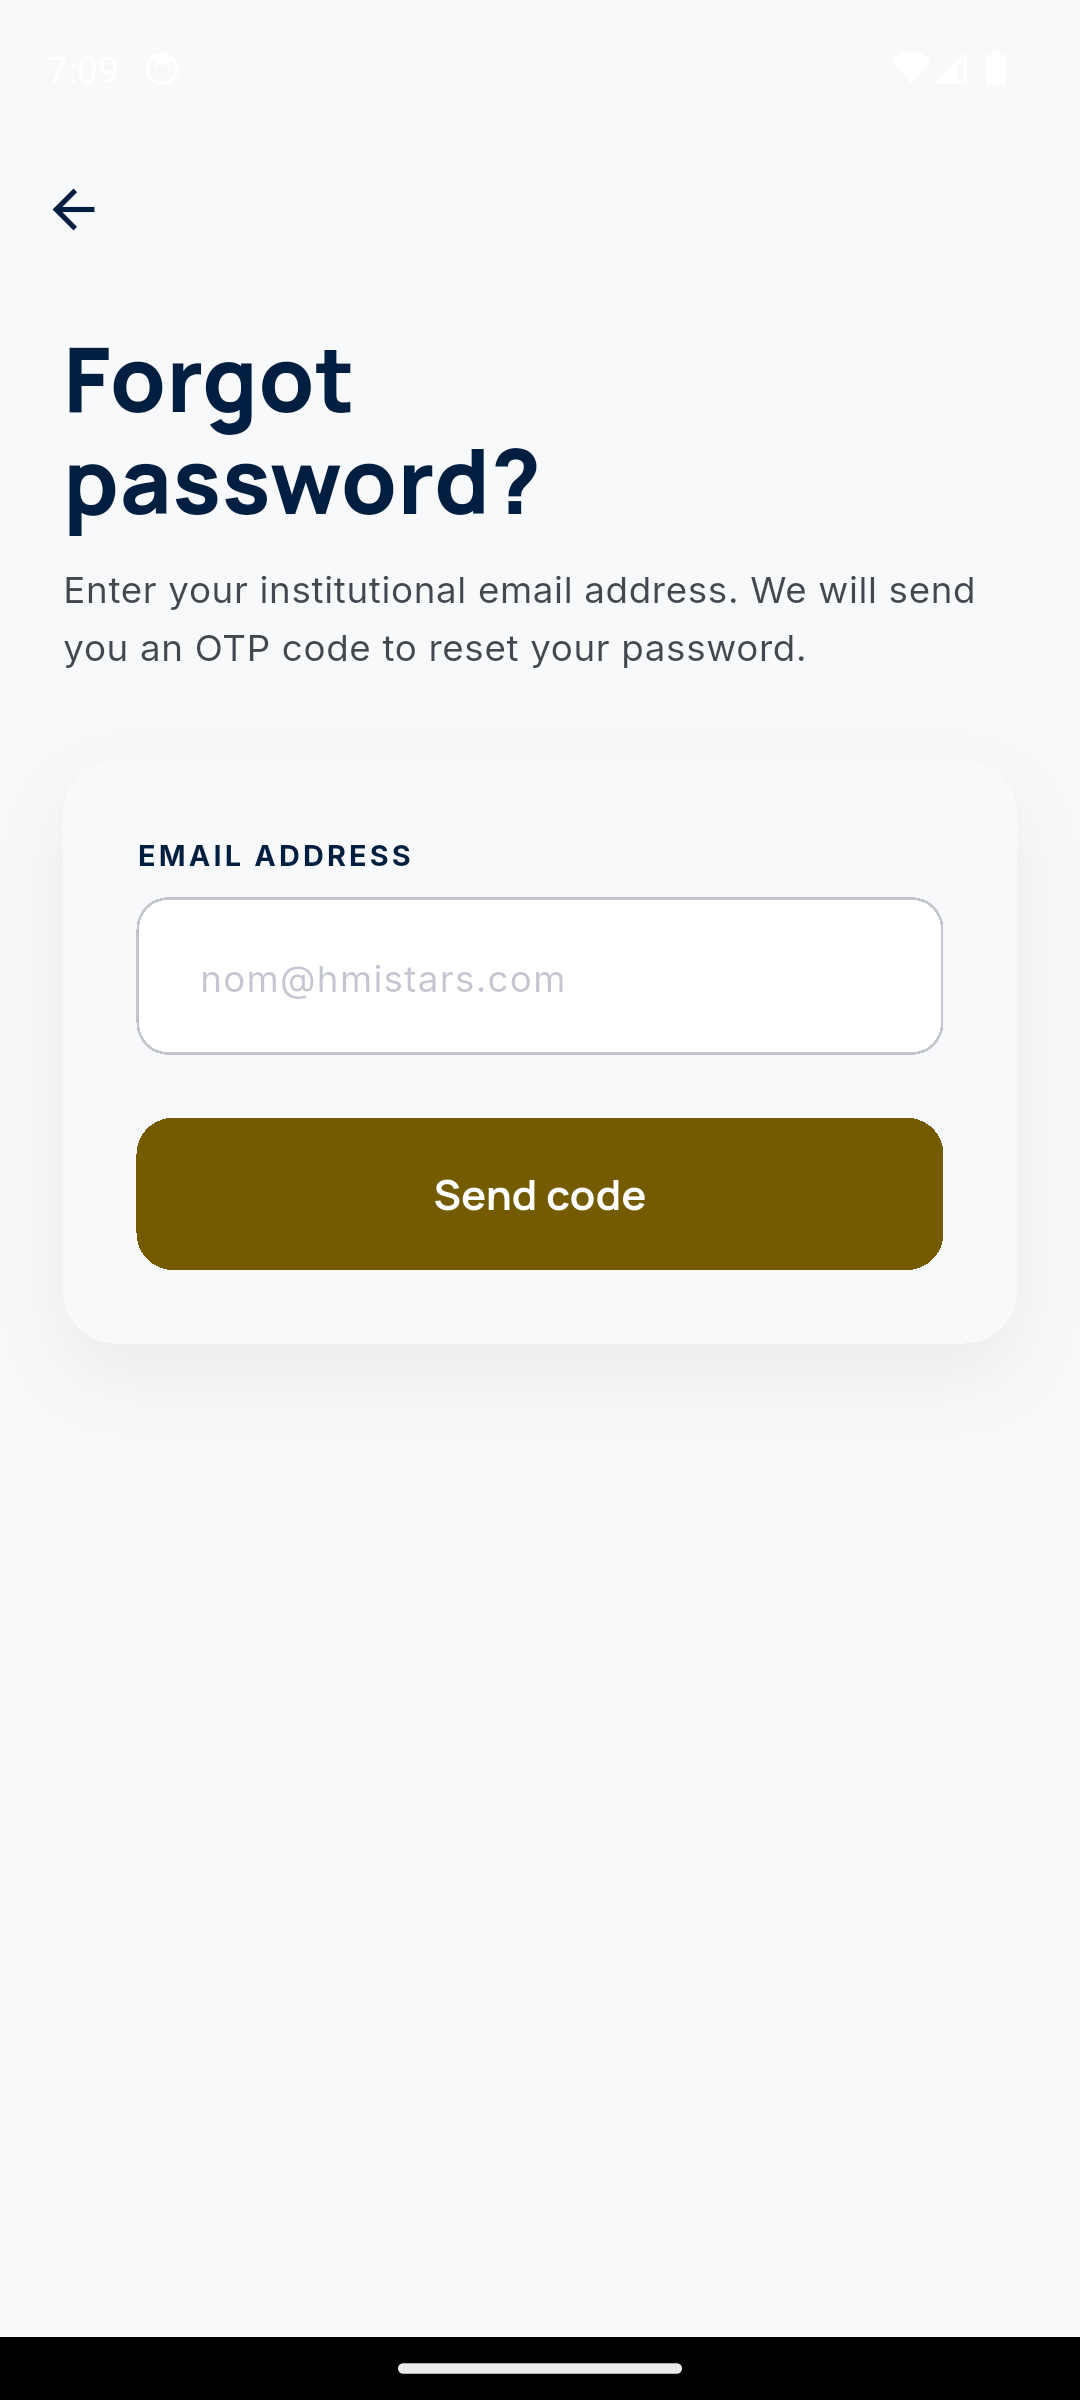
\includegraphics[width=\textwidth]{project_images/App_light_and_english/pass_forget_app.png}
        \caption{Password Forget}
        \label{fig:m_password_forget}
    \end{subfigure}
    \begin{subfigure}[b]{0.24\textwidth}
        \centering
        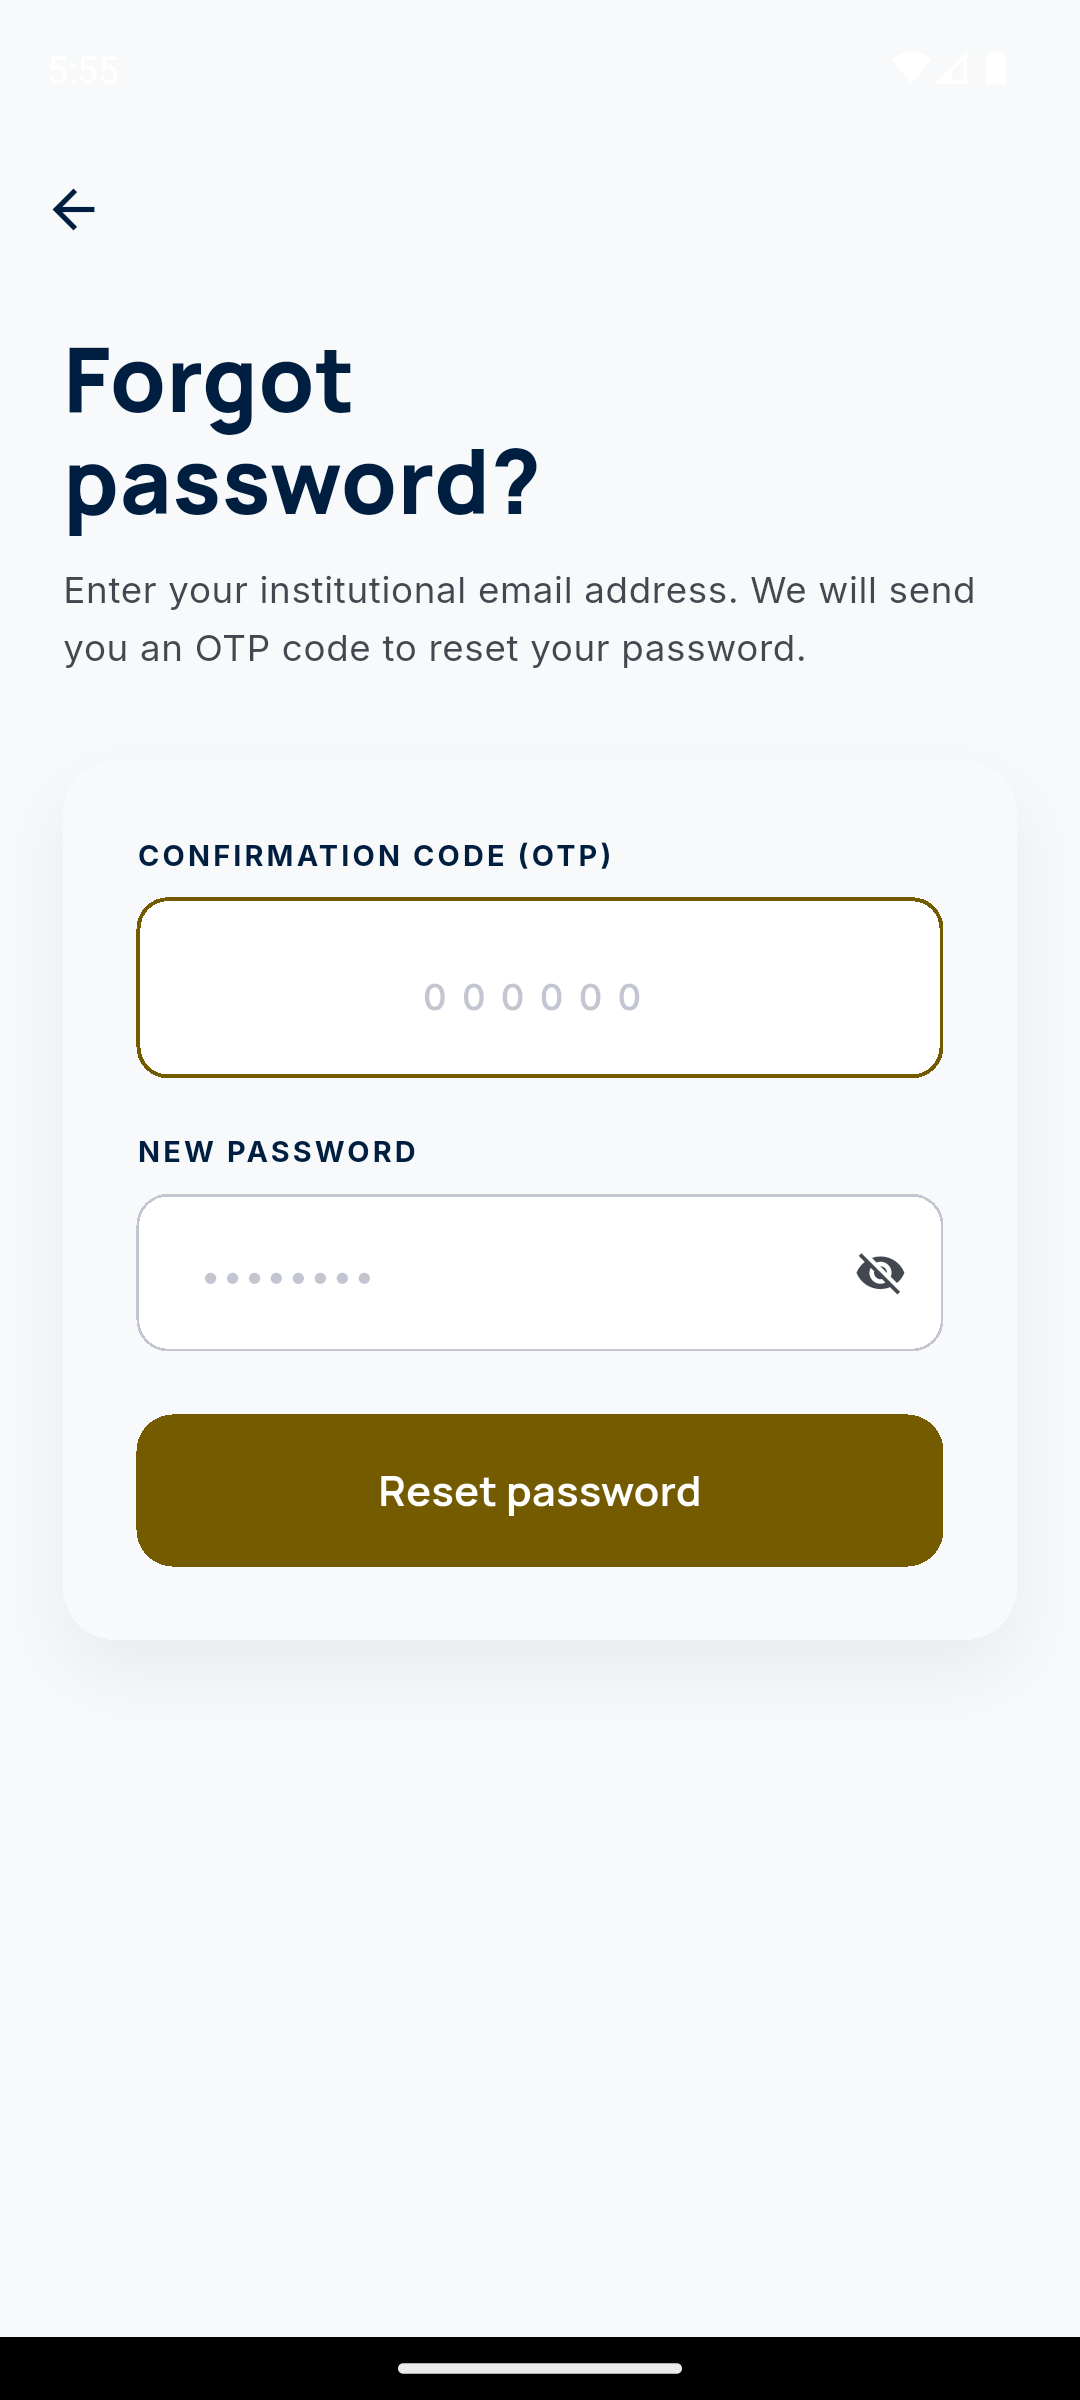
\includegraphics[width=\textwidth]{project_images/App_light_and_english/otp_password_reset.png}
        \caption{Password Reset OTP}
        \label{fig:m_otp_reset}
    \end{subfigure}
    \begin{subfigure}[b]{0.24\textwidth}
        \centering
        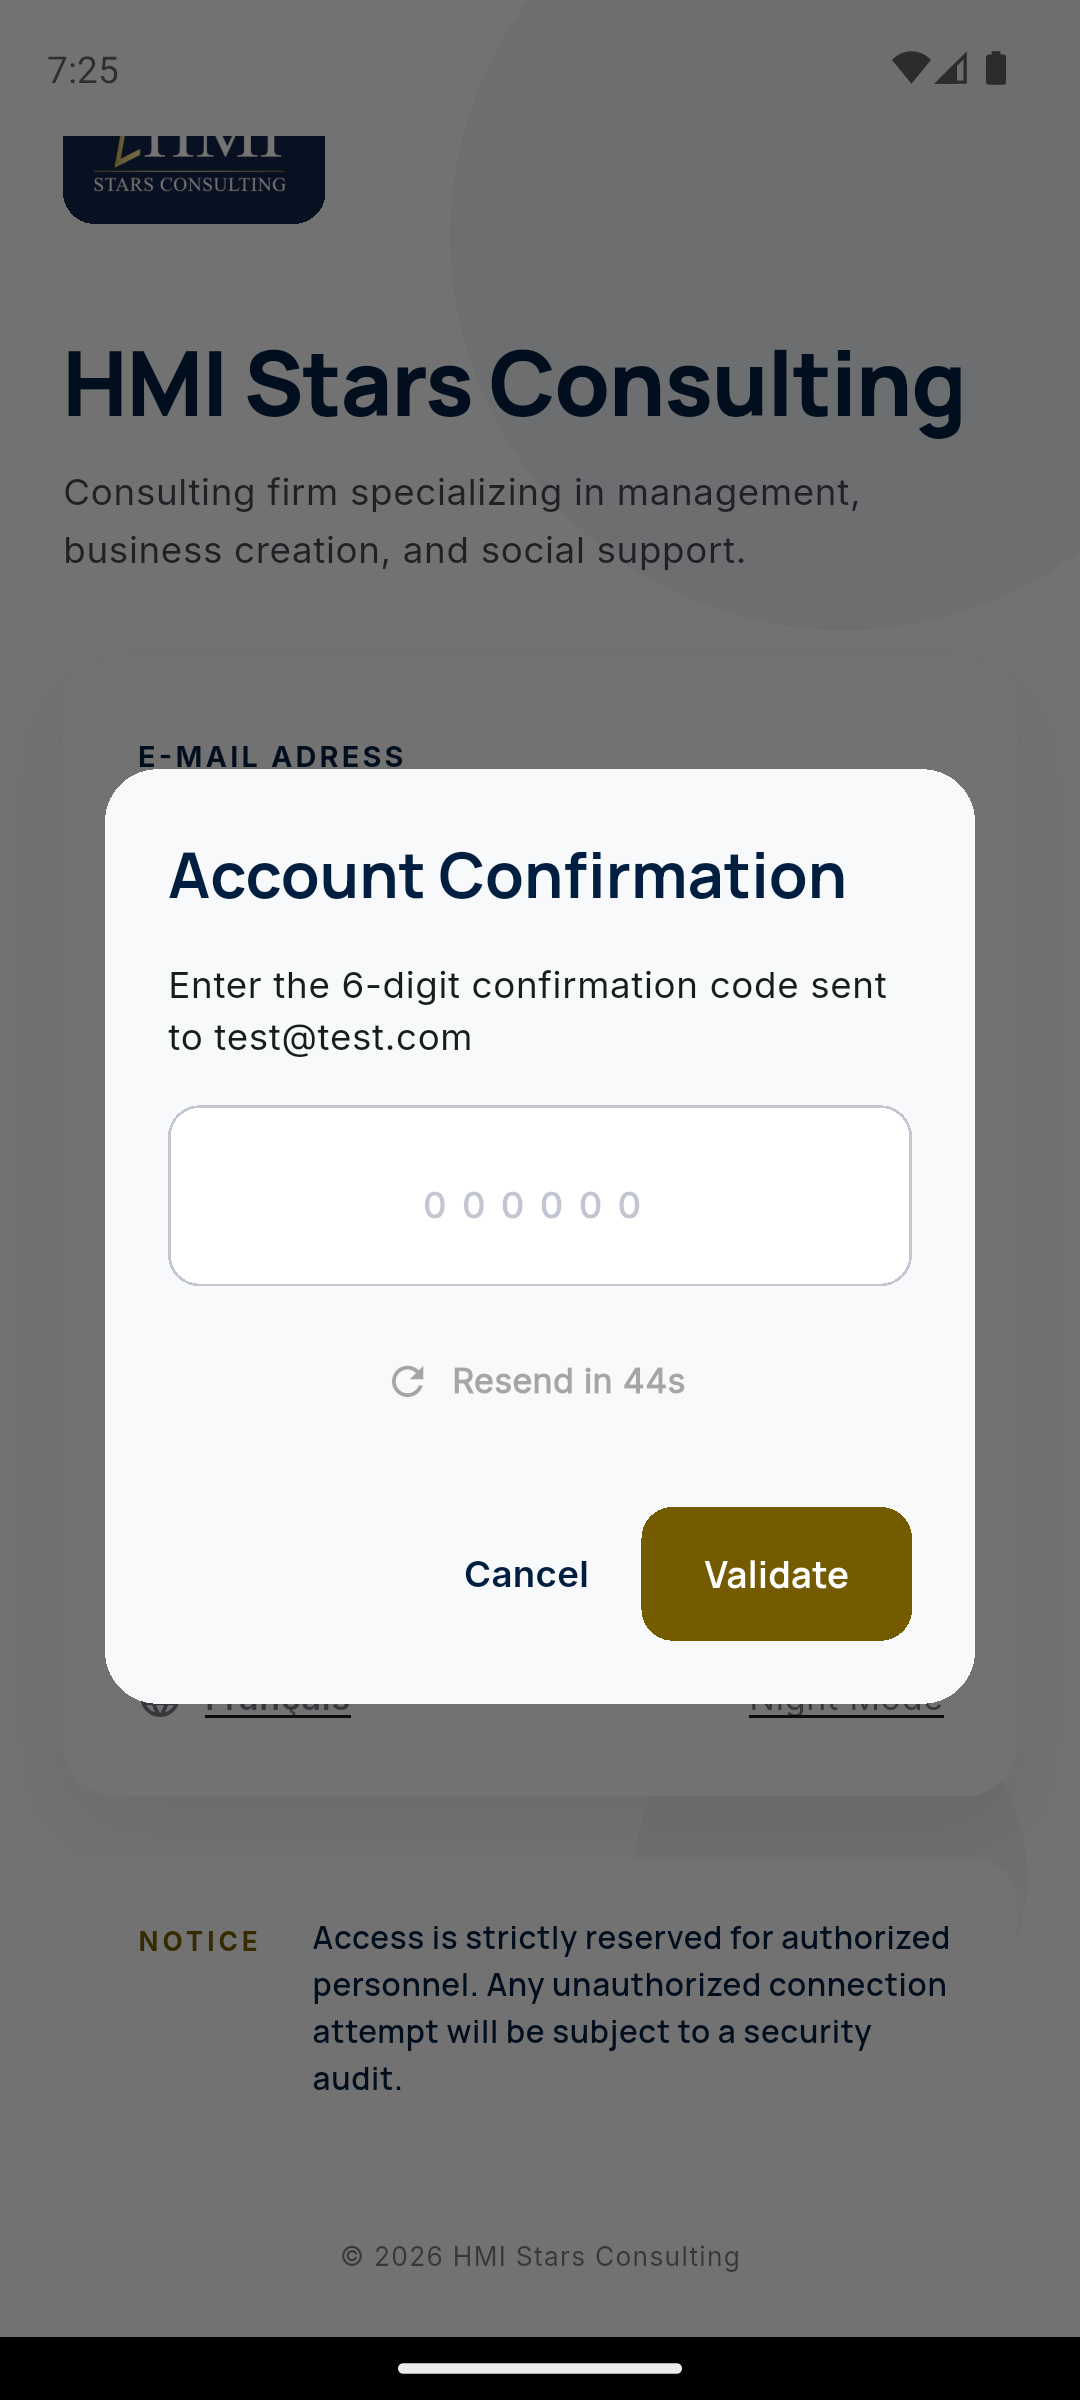
\includegraphics[width=\textwidth]{project_images/App_light_and_english/otp_login_confirmation.png}
        \caption{Confirmation Dialog}
        \label{fig:m_login_otp}
    \end{subfigure}
    \caption{Mobile Application - Authentication, Password Reset and OTP Flows}
    \label{fig:mobile_auth_flow}
\end{figure}

\paragraph{Company Selection and Main Dashboard}
Once authenticated, managers associate their session with a specific enterprise. Figure \ref{fig:mobile_dashboard_flow} shows the Company Selector screen and the main analytical Dashboard workspace, which features metric highlights and a pulsating warning alerts panel.

\begin{figure}[H]
    \centering
    \begin{subfigure}[b]{0.48\textwidth}
        \centering
        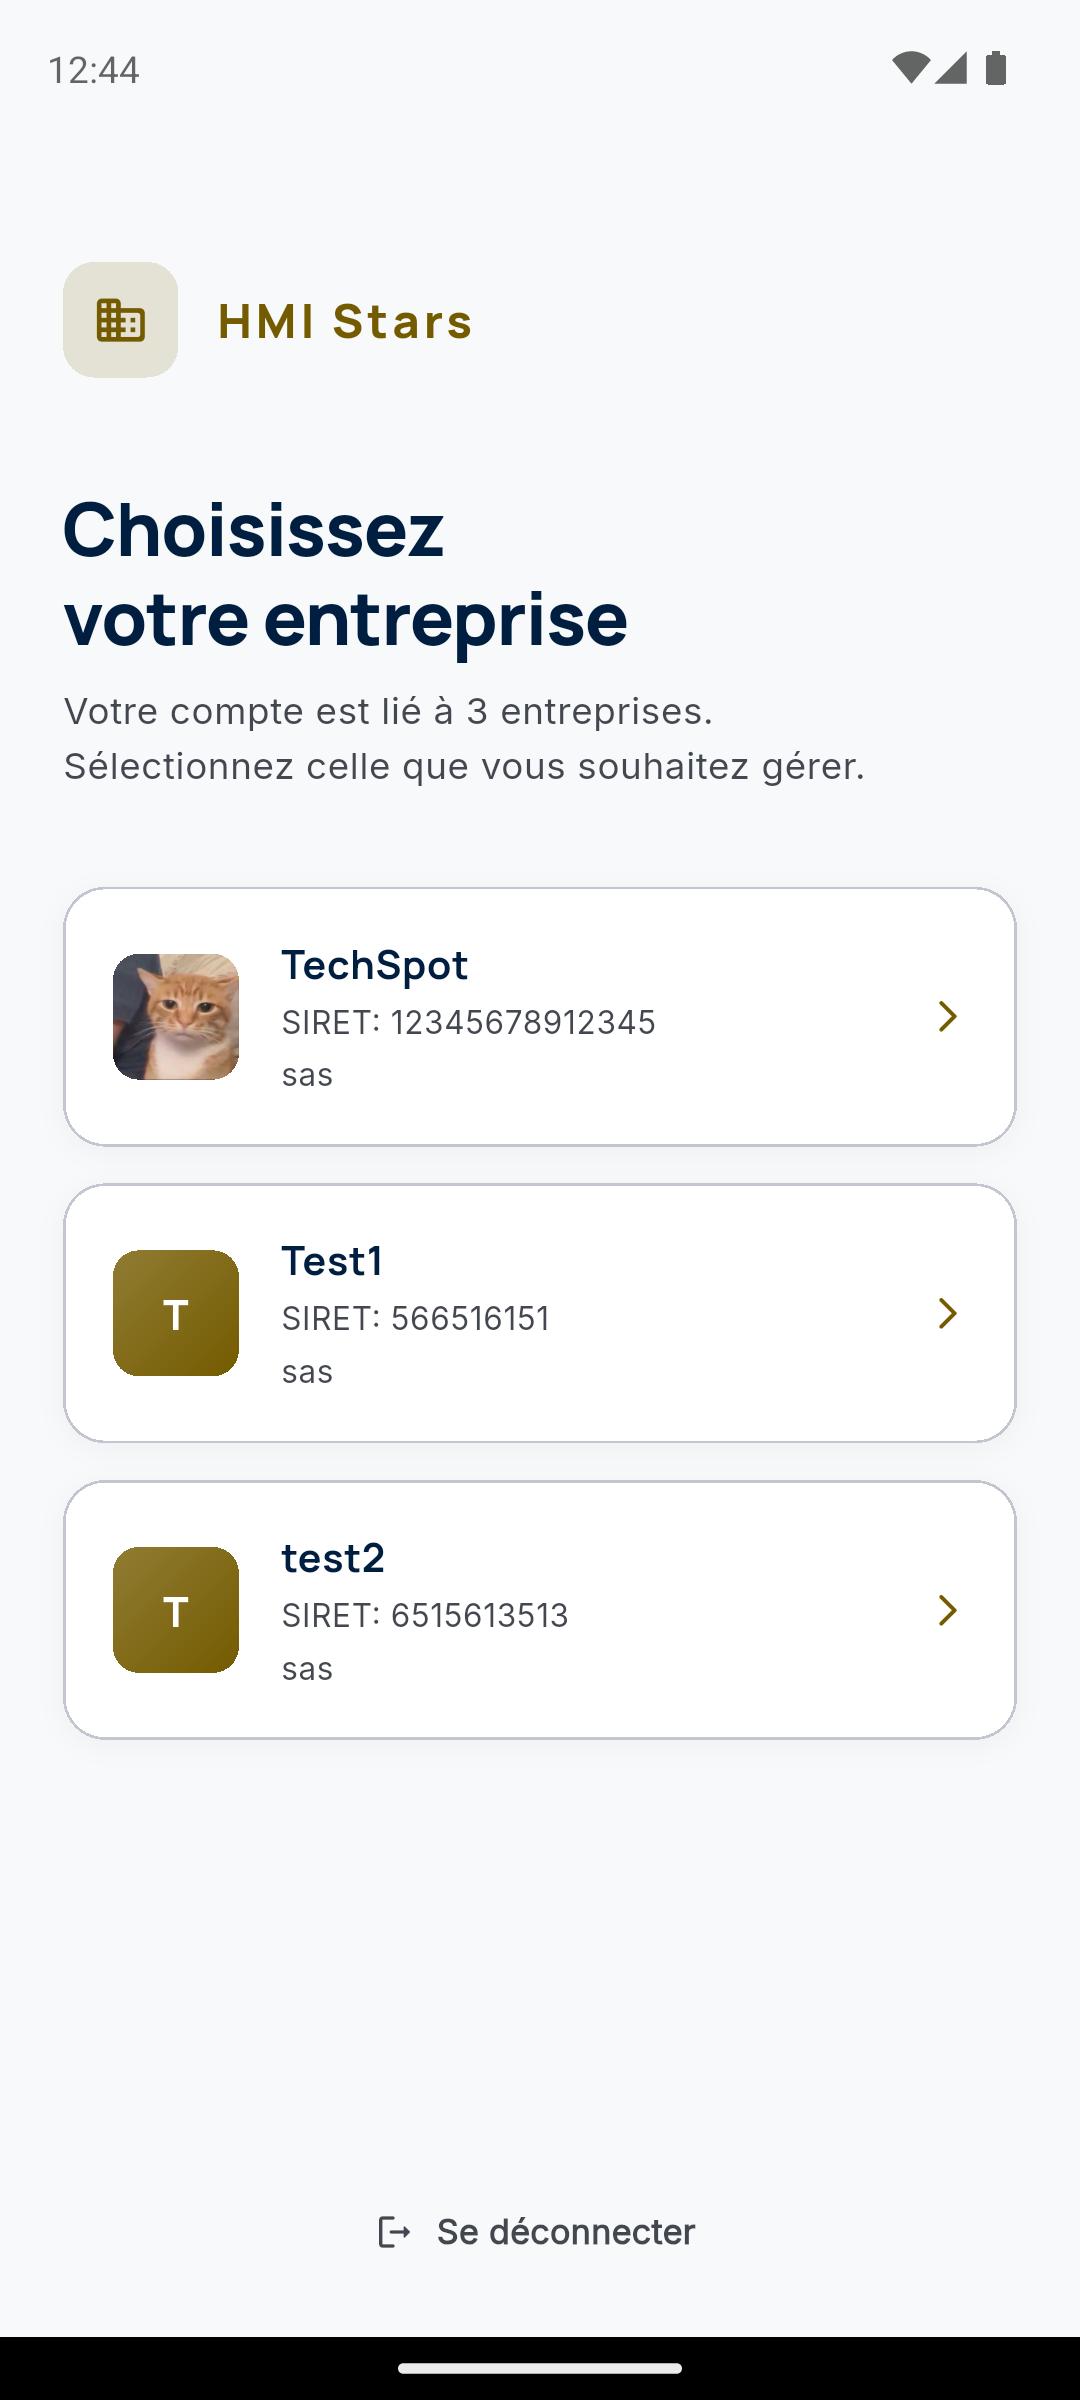
\includegraphics[width=\textwidth]{project_images/company_select.png}
        \caption{Company Selector}
        \label{fig:m_company_selection}
    \end{subfigure}
    \hfill
    \begin{subfigure}[b]{0.48\textwidth}
        \centering
        
\includegraphics[width=\textwidth]{project_images/App_light_and_english/flutter_03.png}
        \caption{Dashboard Overview}
        \label{fig:m_dashboard}
    \end{subfigure}
    \caption{Mobile Application - Company Selection and Dashboard Interfaces}
    \label{fig:mobile_dashboard_flow}
\end{figure}

\paragraph{Pointage \& Attendance Logging}
The daily attendance tracking flow is shown in Figure \ref{fig:mobile_pointage}. It provides a calendar overview, an employee attendance grid, check-in options with note logs, and absence declaration popups.

\begin{figure}[H]
    \centering
    \begin{subfigure}[b]{0.32\textwidth}
        \centering
        
\includegraphics[width=\textwidth]{project_images/App_light_and_english/flutter_04.png}
        \caption{Calendar}
        \label{fig:attendance_cal}
    \end{subfigure}
    \hfill
    \begin{subfigure}[b]{0.32\textwidth}
        \centering
        
\includegraphics[width=\textwidth]{project_images/App_light_and_english/flutter_07.png}
        \caption{Month Picker}
        \label{fig:attendance_picker}
    \end{subfigure}
    \hfill
    \begin{subfigure}[b]{0.32\textwidth}
        \centering
        
\includegraphics[width=\textwidth]{project_images/App_light_and_english/flutter_08.png}
        \caption{Check-in List}
        \label{fig:attendance_list}
    \end{subfigure}
    \vspace{0.3cm}
    
    \begin{subfigure}[b]{0.32\textwidth}
        \centering
        
\includegraphics[width=\textwidth]{project_images/App_light_and_english/flutter_10.png}
        \caption{Notes Dialog}
        \label{fig:attendance_notes}
    \end{subfigure}
    \hfil
    \begin{subfigure}[b]{0.32\textwidth}
        \centering
        
\includegraphics[width=\textwidth]{project_images/App_light_and_english/flutter_09.png}
        \caption{Absence Form}
        \label{fig:m_abs_form}
    \end{subfigure}
    \caption{Mobile Application - Daily Activity Attendance Tracking Flow}
    \label{fig:mobile_pointage}
\end{figure}

\paragraph{Leaves and Absences Requests}
The leaves and absences request subsystem allows managers to declare absences and submit leave requests. Figure \ref{fig:mobile_leaves} shows the interface where requests are registered along with justifications and descriptive notes.

\begin{figure}[H]
    \centering
    \begin{subfigure}[b]{0.48\textwidth}
        \centering
        
\includegraphics[width=\textwidth]{project_images/App_light_and_english/flutter_06.png}
        \caption{Leaves List View}
        \label{fig:m_leaves_list}
    \end{subfigure}
    \hfill
    \begin{subfigure}[b]{0.48\textwidth}
        \centering
        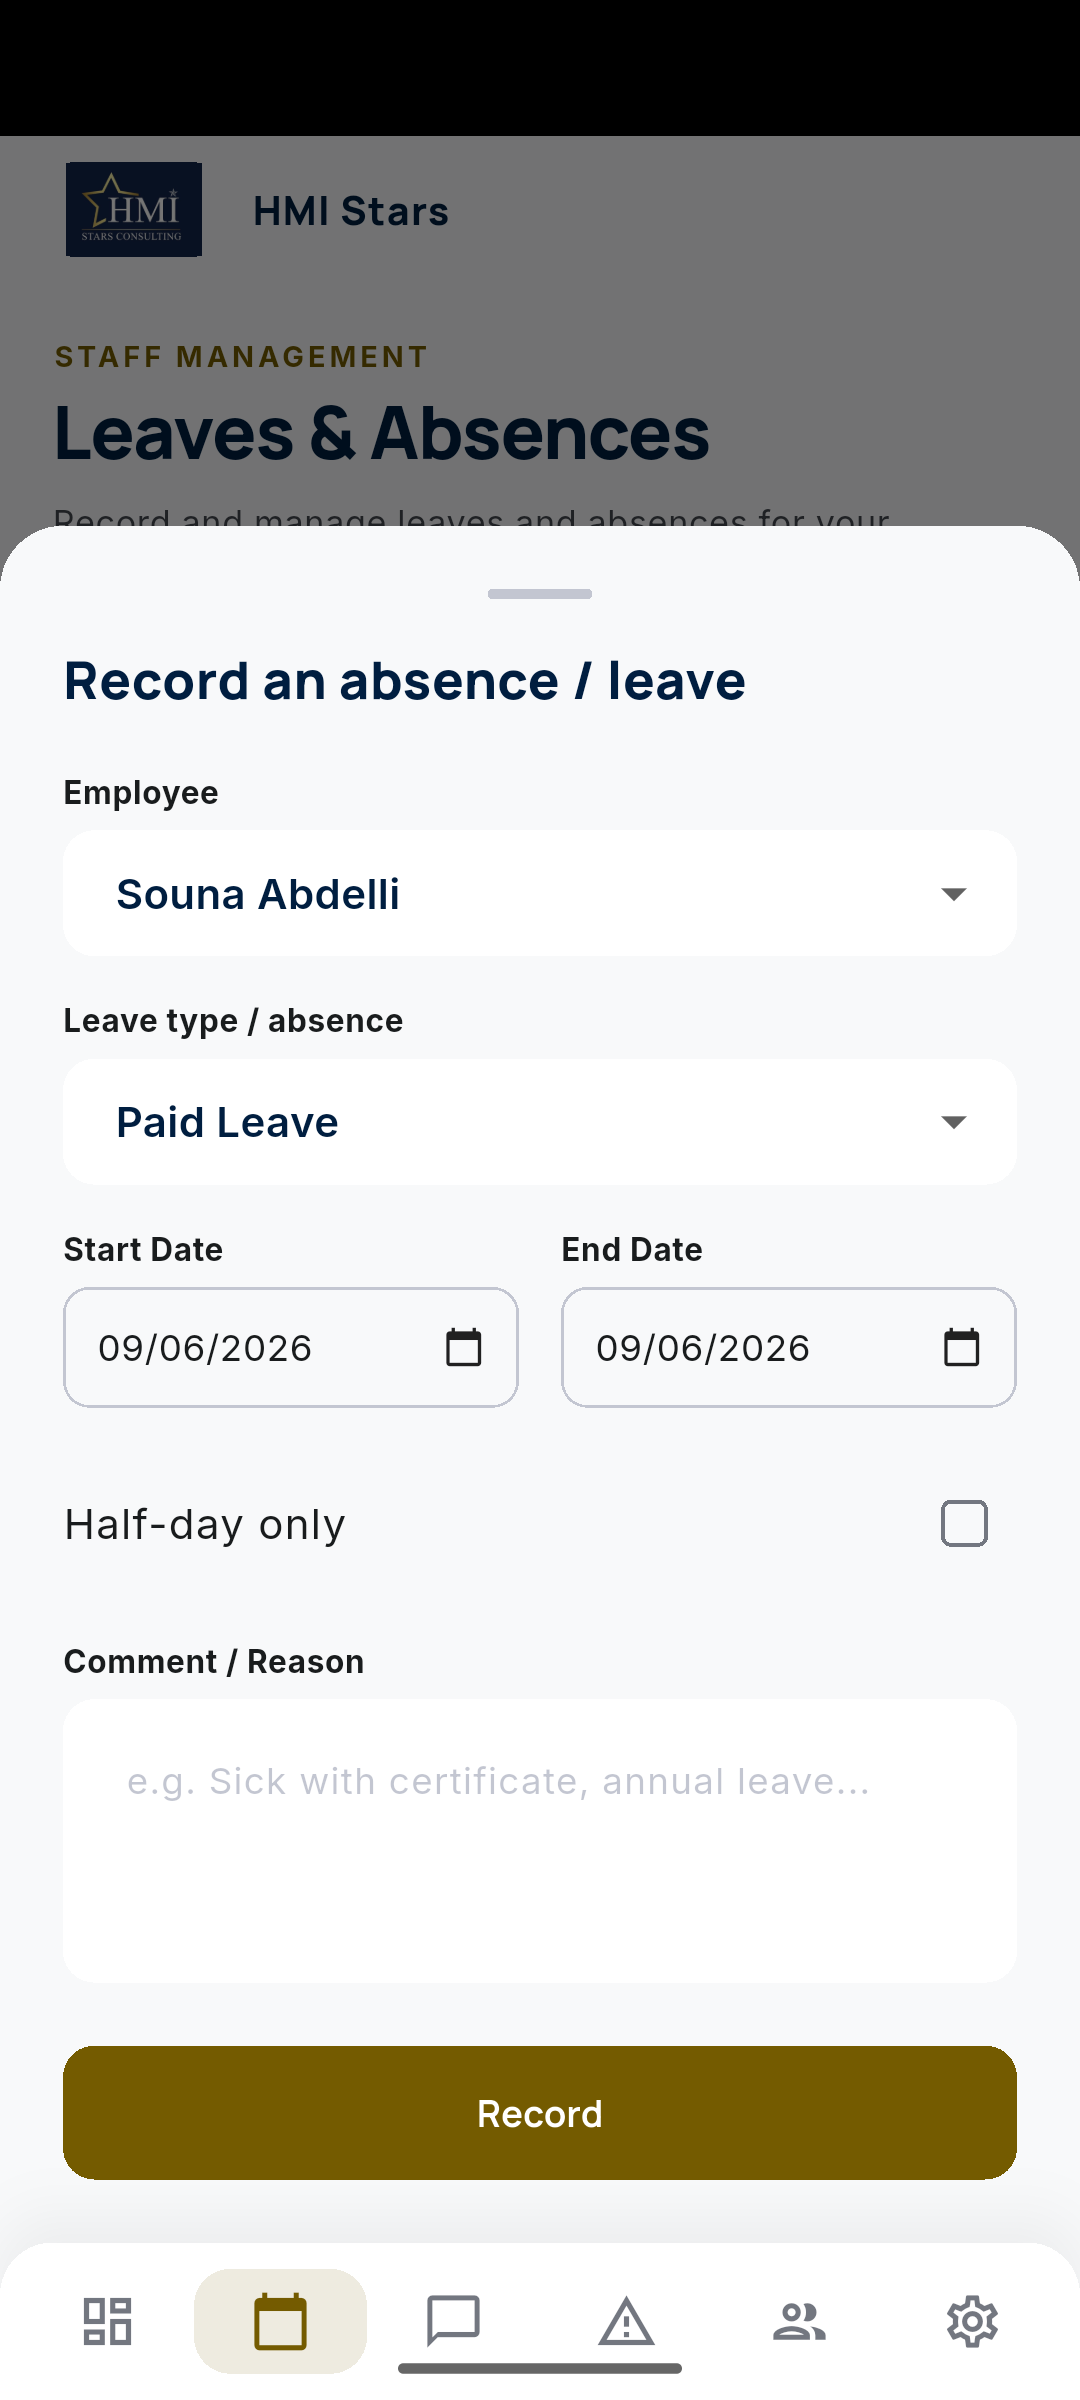
\includegraphics[width=\textwidth]{project_images/App_light_and_english/flutter_07_1.png}
        \caption{Leave Declaration Form}
        \label{fig:m_leaves_form}
    \end{subfigure}
    \caption{Mobile Application - Leaves and Absences Management}
    \label{fig:mobile_leaves}
\end{figure}

\paragraph{Support Chat and Media Attachment Drawer}
Real-time chat and document sharing interfaces allow direct communication with HMI Stars managers. As displayed in Figure \ref{fig:mobile_chat}, this includes the support chat, a list of shared files, and real-time scanned document attachment previews.

\begin{figure}[H]
    \centering

    \begin{subfigure}[b]{0.24\textwidth}
        \centering
        
\includegraphics[width=\textwidth]{project_images/App_light_and_english/flutter_11.png}
        \caption{Contacts}
        \label{fig:m_contacts}
    \end{subfigure}
    \begin{subfigure}[b]{0.24\textwidth}
        \centering
        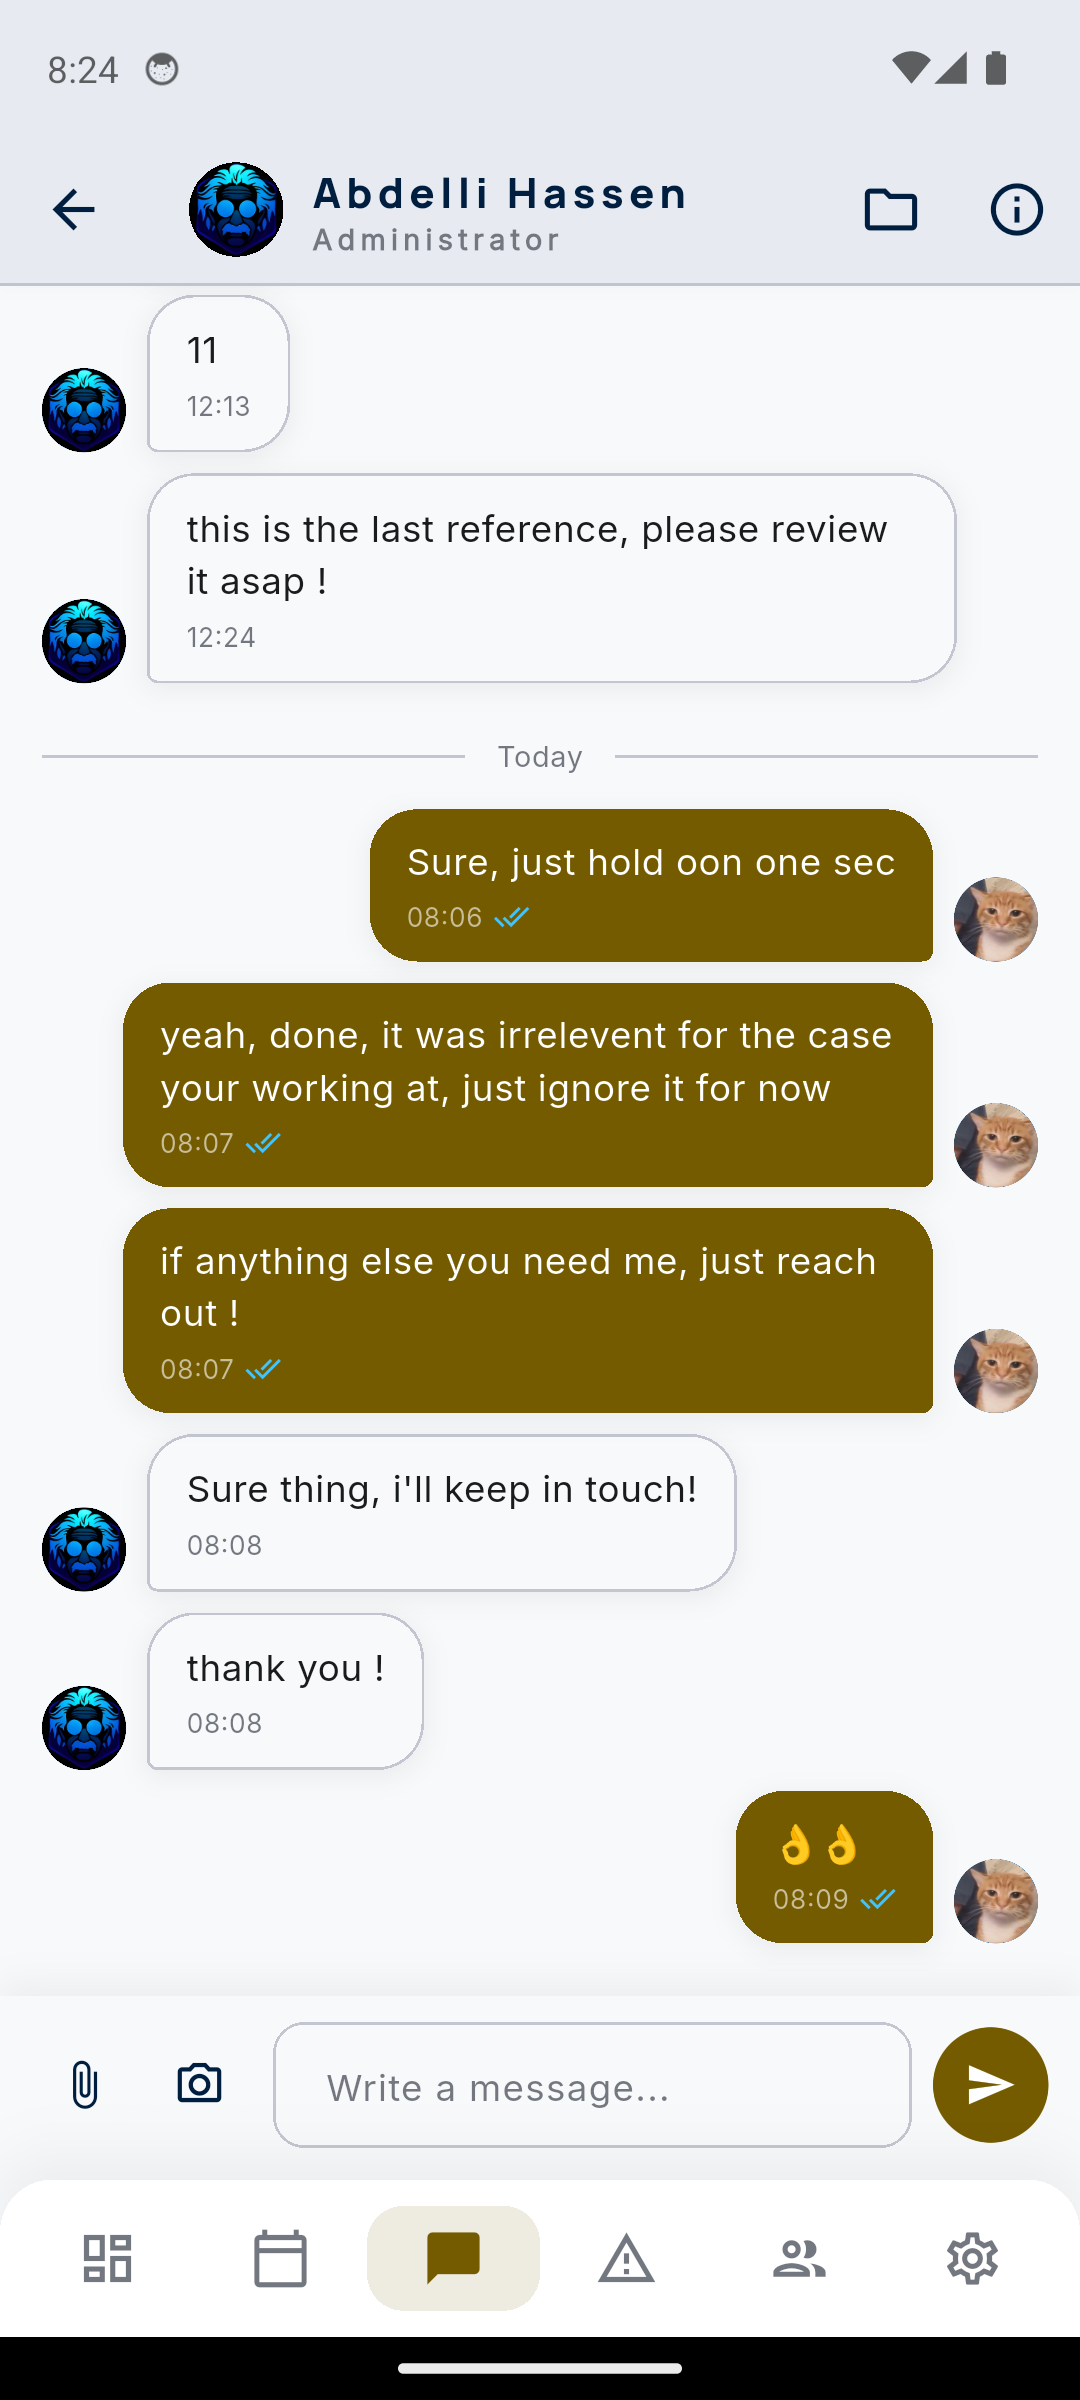
\includegraphics[width=\textwidth]{project_images/App_light_and_english/chat.png}
        \caption{Chat}
        \label{fig:m_chat}
    \end{subfigure}
    \begin{subfigure}[b]{0.24\textwidth}
        \centering
        
\includegraphics[width=\textwidth]{project_images/App_light_and_english/flutter_13.png}
        \caption{Attachment Preview}
        \label{fig:m_attachment_preview}
    \end{subfigure}
    \begin{subfigure}[b]{0.24\textwidth}
        \centering
        
\includegraphics[width=\textwidth]{project_images/App_light_and_english/flutter_15.png}
        \caption{Shared Files}
        \label{fig:m_docs}
    \end{subfigure}

    \caption{Mobile Application - Chats, Contacts, and Shared Document Panels}
    \label{fig:mobile_chat}
\end{figure}

\paragraph{Employee Directory Views}
The employee management module allows company managers to view active and archived employees directly from the mobile application. Figure \ref{fig:mobile_employee_views} shows the employee directory in both grid and list view modes.

\begin{figure}[H]
    \centering
    \begin{subfigure}[b]{0.41\textwidth}
        \centering
        
\includegraphics[width=0.7\textwidth]{project_images/App_light_and_english/flutter_20.png}
        \caption{Grid View}
        \label{fig:m_emp_grid}
    \end{subfigure}
    \begin{subfigure}[b]{0.41\textwidth}
        \centering
        
\includegraphics[width=0.7\textwidth]{project_images/App_light_and_english/flutter_25.png}
        \caption{List View}
        \label{fig:m_emp_list}
    \end{subfigure}
    \caption{Mobile Application - Employee Directory Views}
    \label{fig:mobile_employee_views}
\end{figure}

\paragraph{Employee Profile Operations}
To add, consult, or edit employee records, managers use the dedicated profiling interfaces. Figure \ref{fig:mobile_employee_ops} shows the new employee registration form, the detailed profile file, and the profile editing interface.

\begin{figure}[H]
    \centering
    \begin{subfigure}[b]{0.32\textwidth}
        \centering
        
\includegraphics[width=\textwidth]{project_images/App_light_and_english/flutter_24.png}
        \caption{New Employee Form}
        \label{fig:m_new_emp}
    \end{subfigure}
    \hfill
    \begin{subfigure}[b]{0.32\textwidth}
        \centering
        
\includegraphics[width=\textwidth]{project_images/App_light_and_english/flutter_21.png}
        \caption{Employee Profile}
        \label{fig:m_emp_profile}
    \end{subfigure}
    \hfill
    \begin{subfigure}[b]{0.32\textwidth}
        \centering
        
\includegraphics[width=\textwidth]{project_images/App_light_and_english/flutter_22.png}
        \caption{Profile Editor}
        \label{fig:m_emp_edit}
    \end{subfigure}
    \caption{Mobile Application - Employee Registration, Detailed Profiling, and Editing Forms}
    \label{fig:mobile_employee_ops}
\end{figure}

\paragraph{Interactive Document Scanner}
To streamline file transmissions, the mobile client embeds an interactive camera-based scanner. Figure \ref{fig:m_scanner_steps} demonstrates the scanner step-by-step: choosing the source, taking a picture, adjusting perspective crop, applying filters, and previewing the document.

\begin{figure}[H]
    \centering
    \begin{subfigure}[b]{0.32\textwidth}
        \centering
        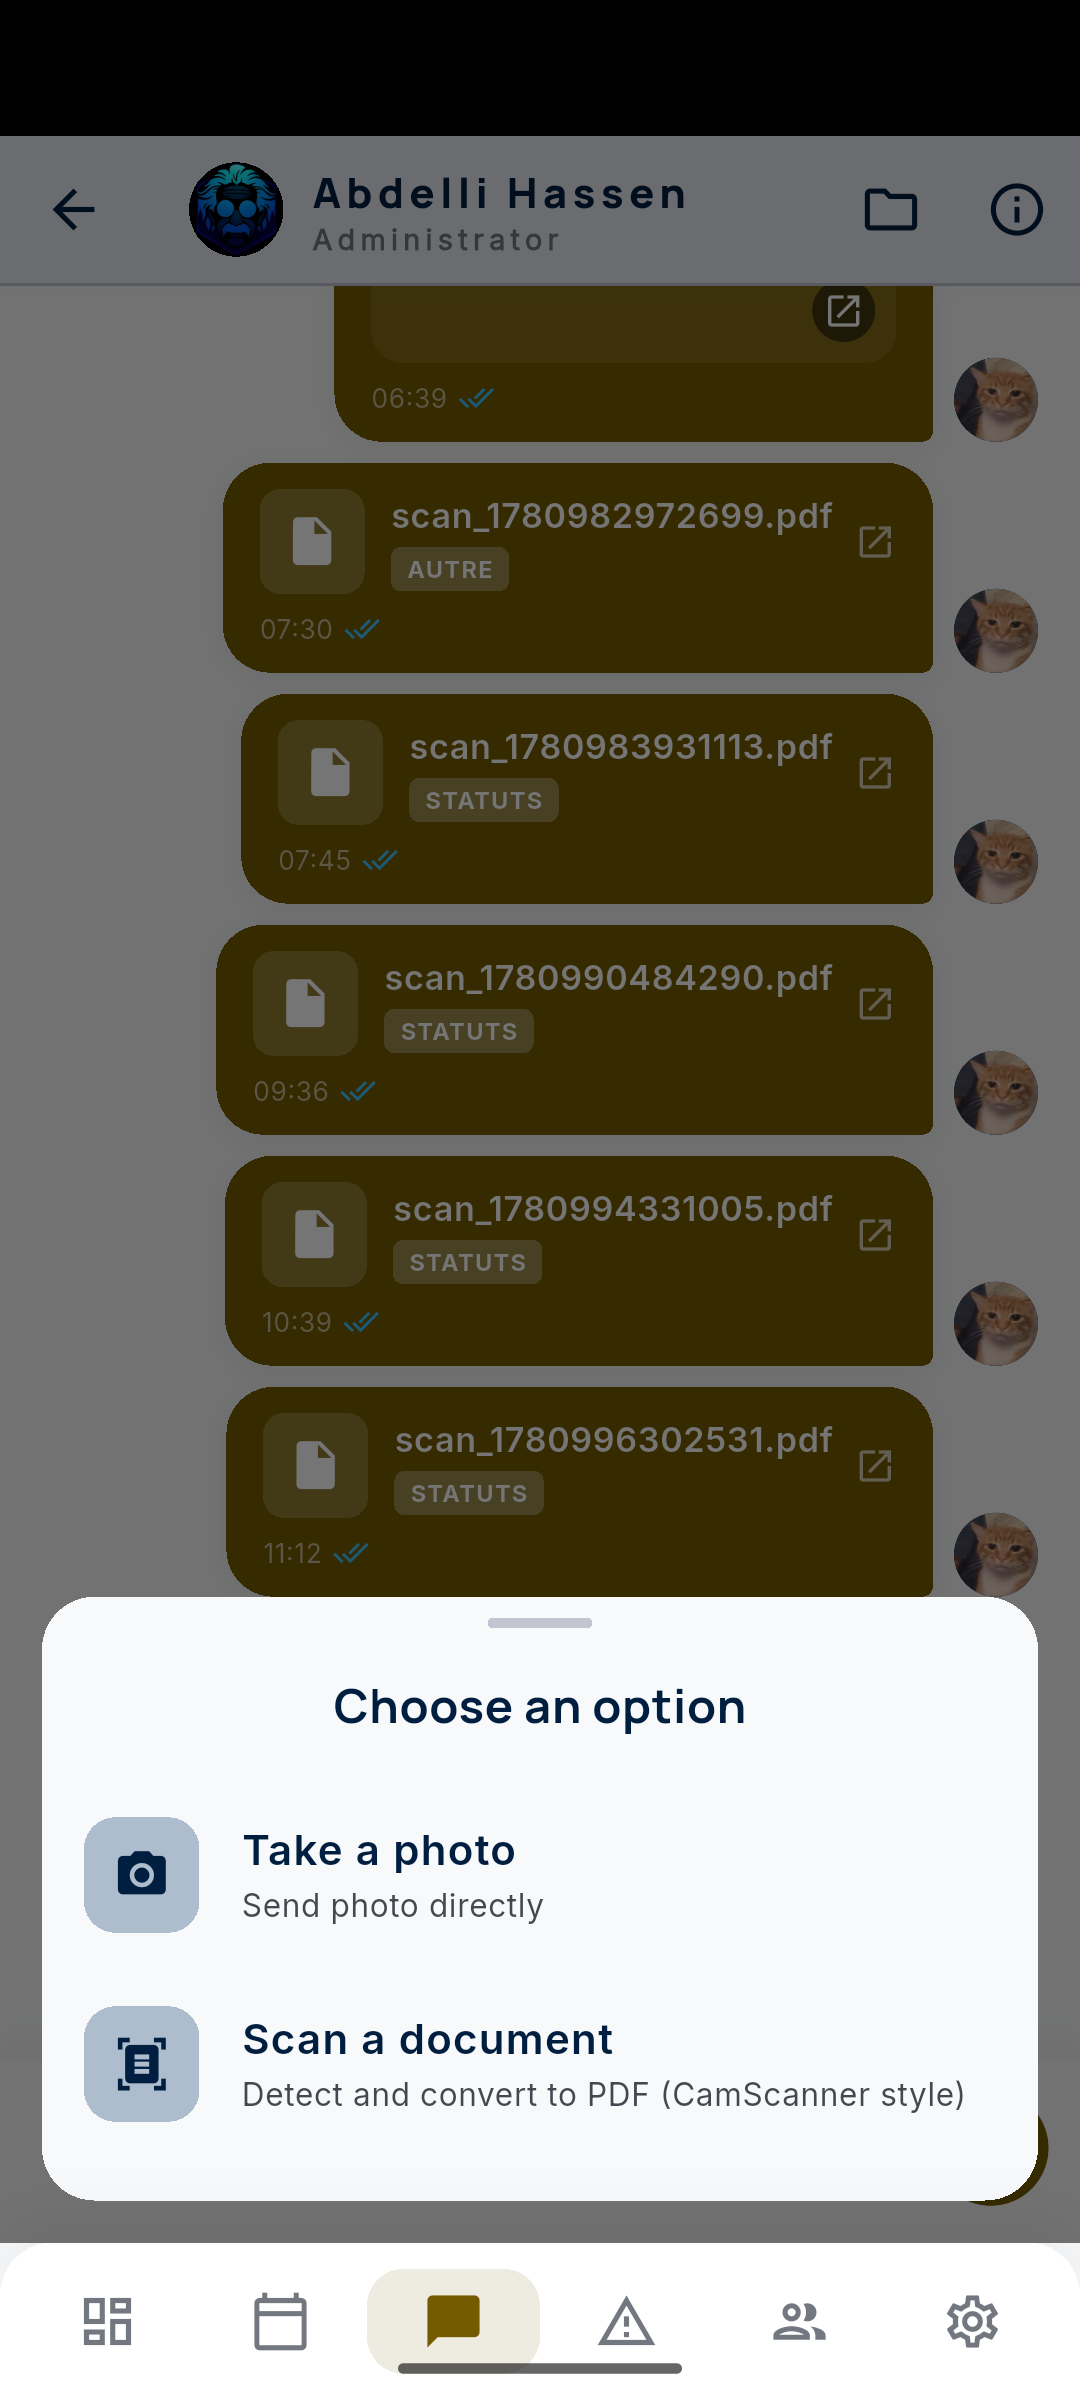
\includegraphics[width=\textwidth]{project_images/App_light_and_english/flutter_01_1.png}
        \caption{Mode Choice}
    \end{subfigure}
    \hfill
    \begin{subfigure}[b]{0.32\textwidth}
        \centering
        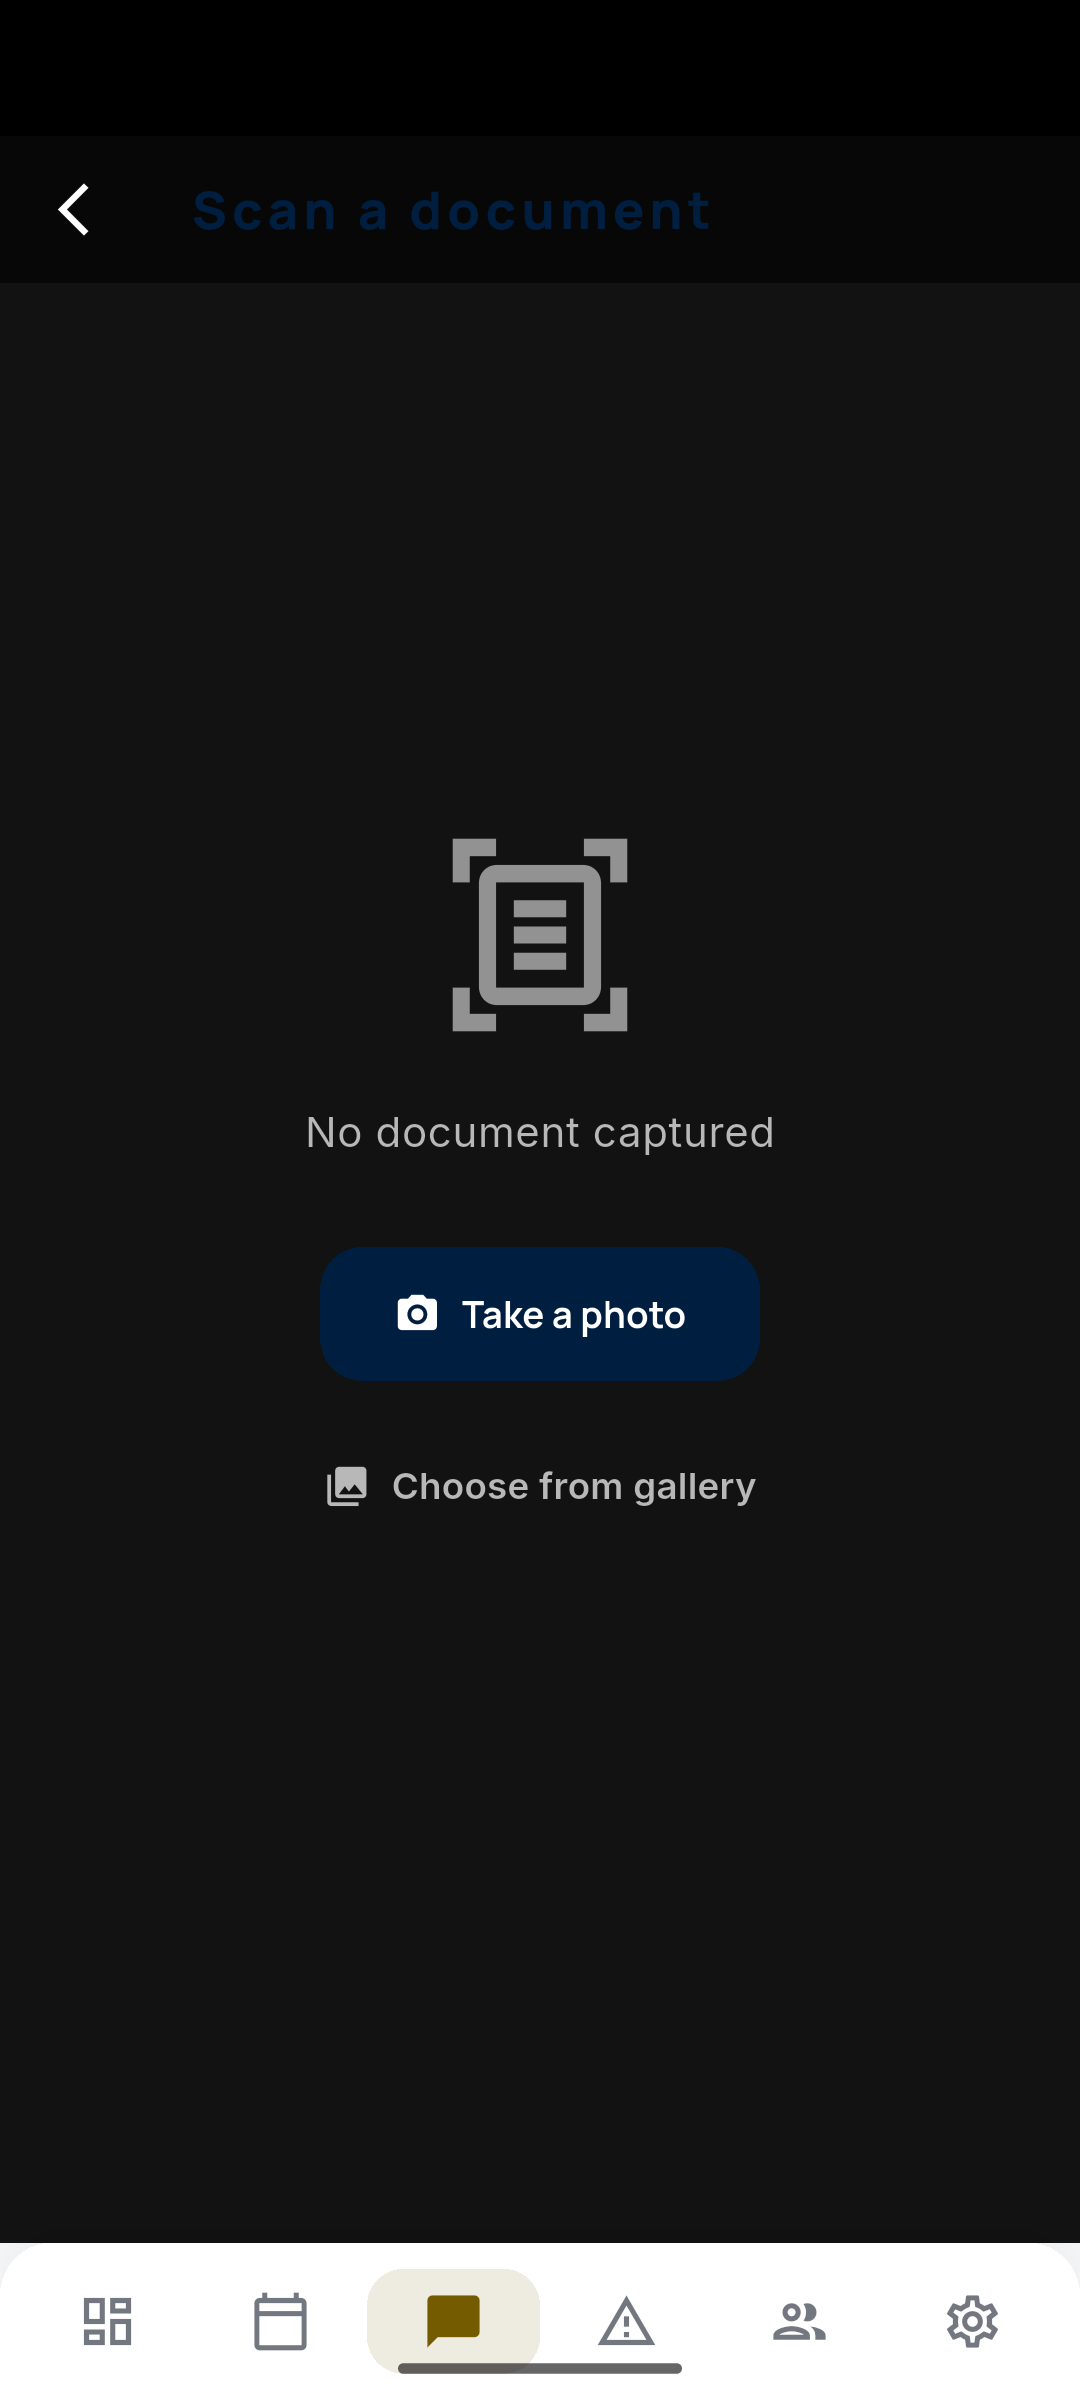
\includegraphics[width=\textwidth]{project_images/App_light_and_english/flutter_02_1.png}
        \caption{Camera View}
    \end{subfigure}
    \hfill
    \begin{subfigure}[b]{0.32\textwidth}
        \centering
        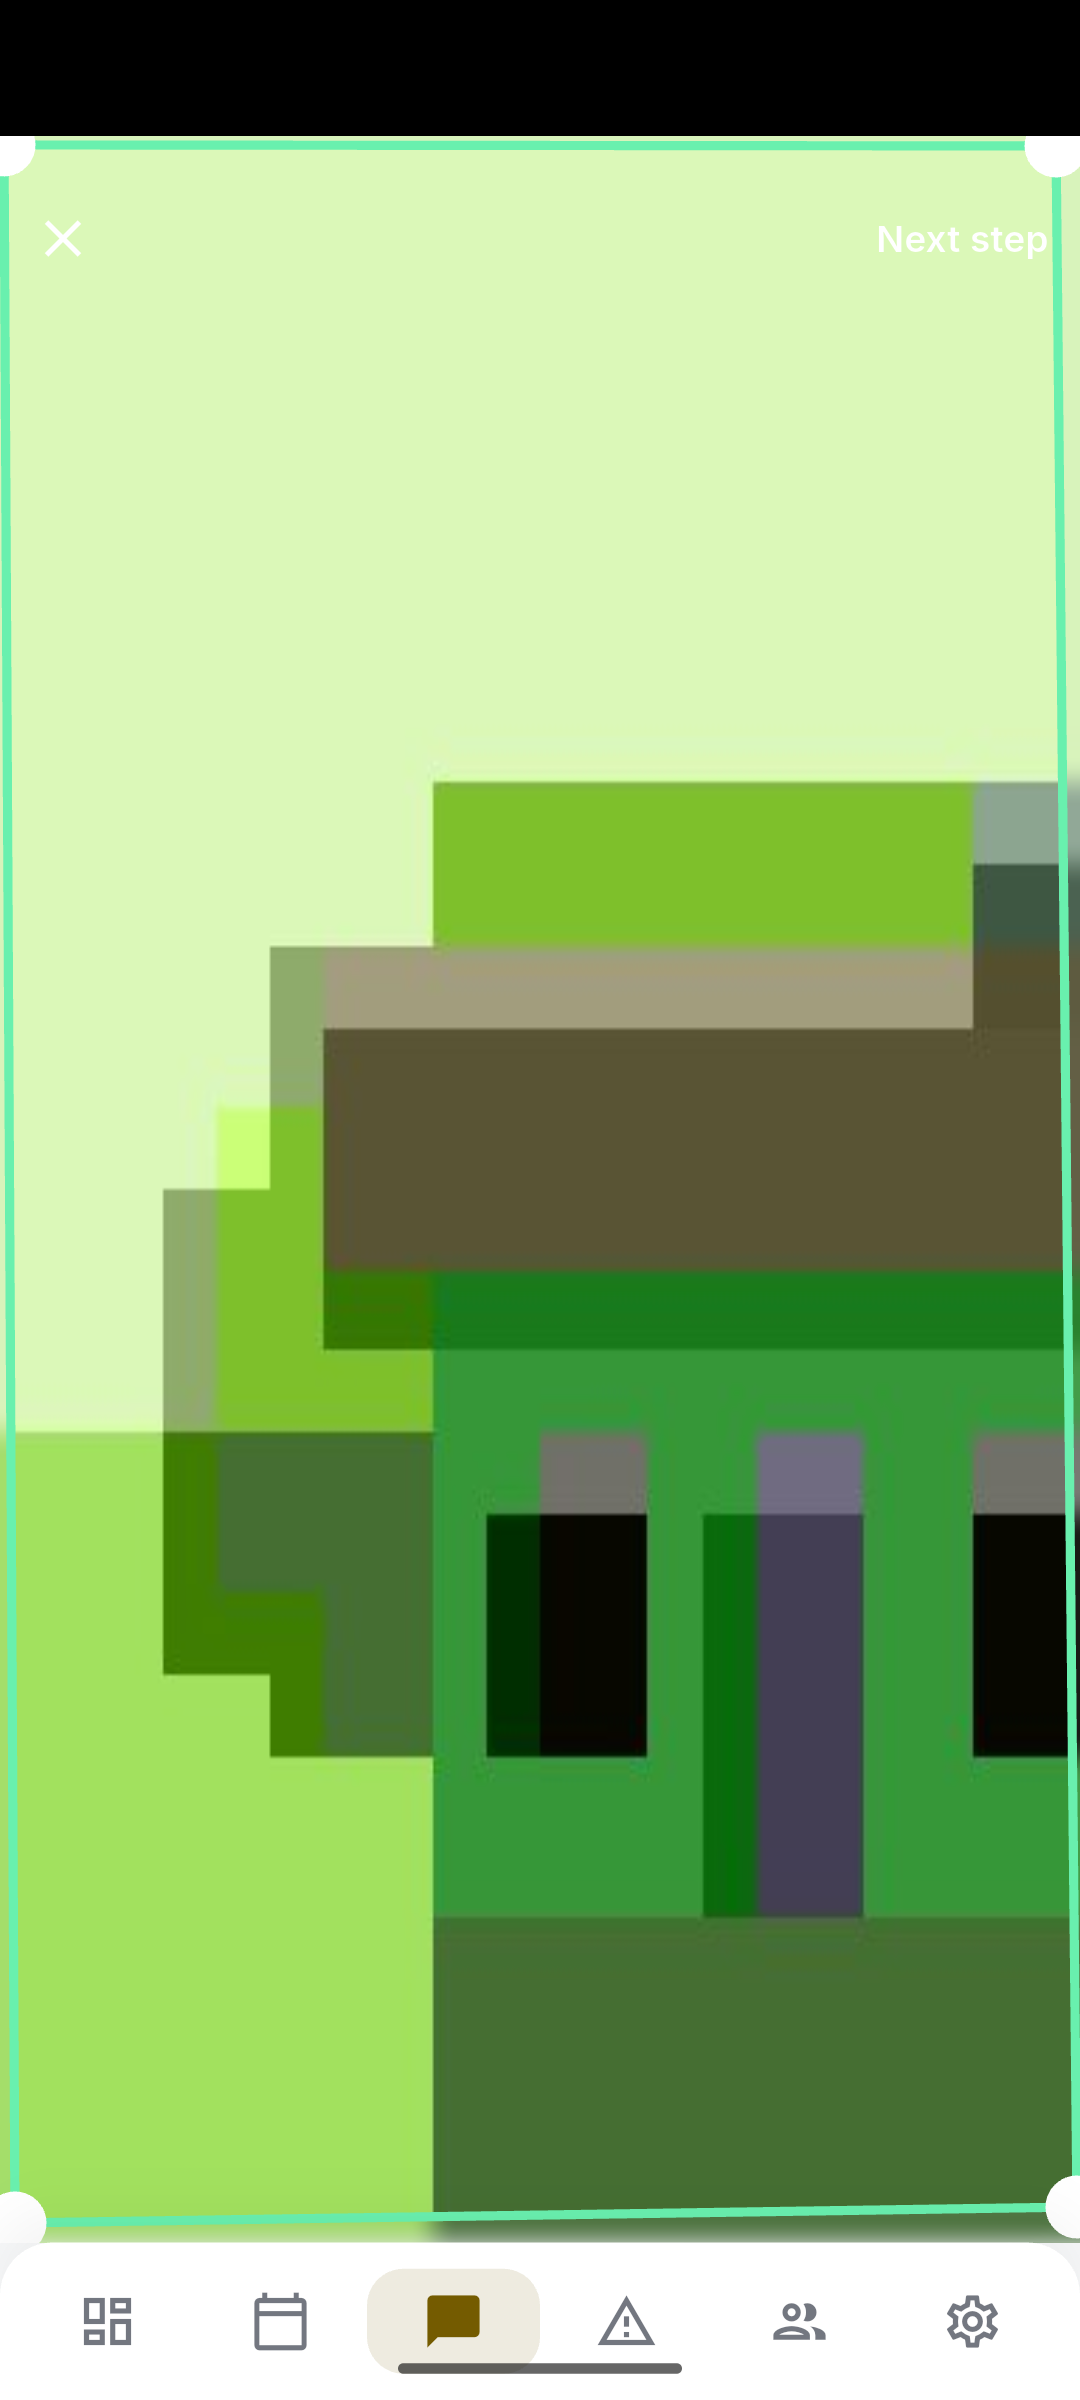
\includegraphics[width=\textwidth]{project_images/App_light_and_english/flutter_03_1.png}
        \caption{Cropping stage}
    \end{subfigure}
    \vspace{0.3cm}

    \begin{subfigure}[b]{0.32\textwidth}
        \centering
        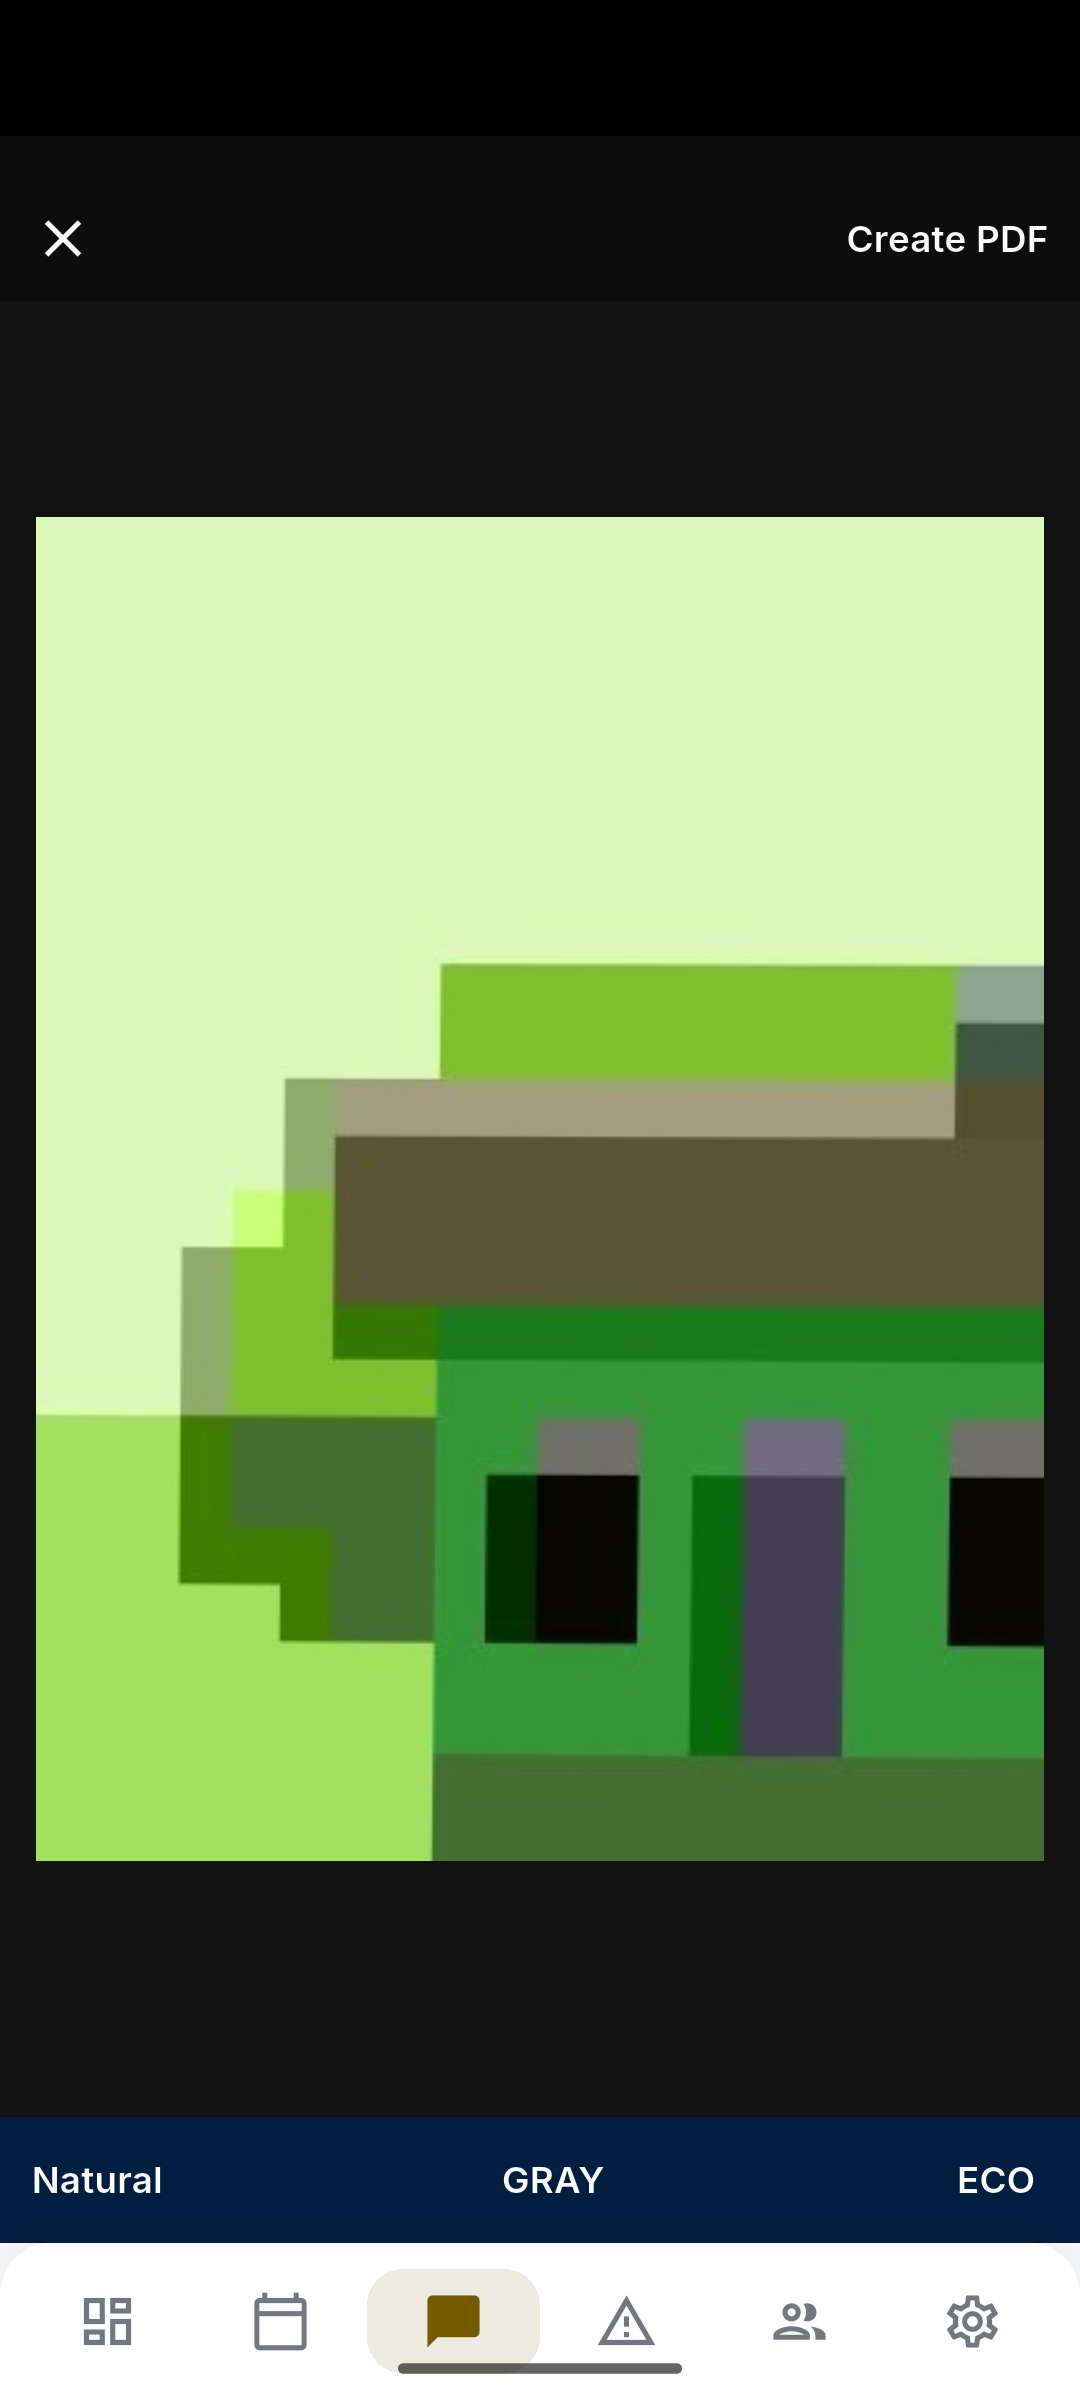
\includegraphics[width=\textwidth]{project_images/App_light_and_english/flutter_04_1.png}
        \caption{Filters Grid}
    \end{subfigure}
    \hfil
    \begin{subfigure}[b]{0.32\textwidth}
        \centering
        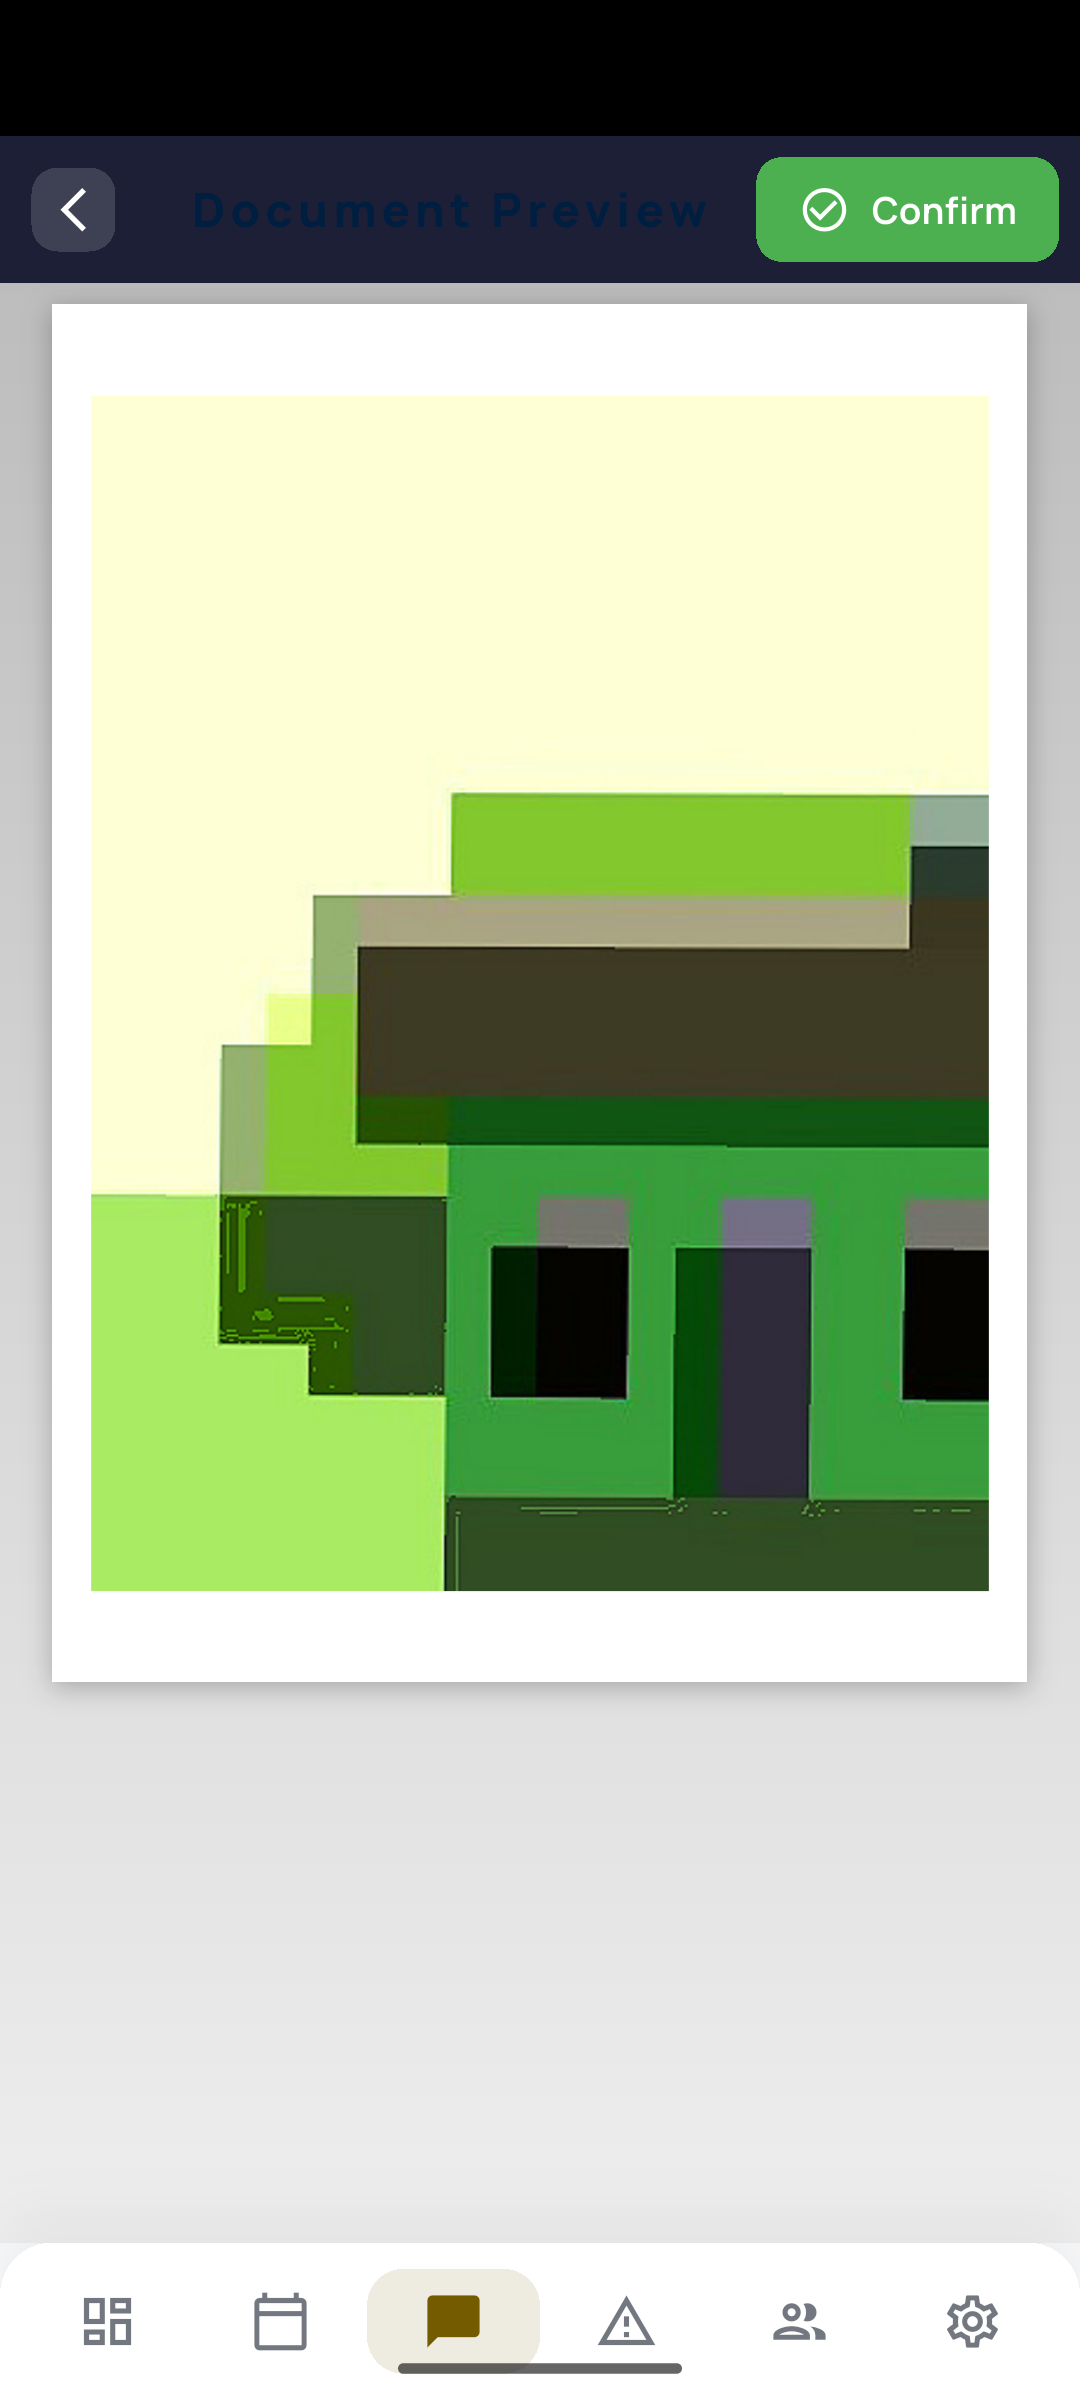
\includegraphics[width=\textwidth]{project_images/App_light_and_english/flutter_05_1.png}
        \caption{Confirm Send}
    \end{subfigure}
    \caption{Mobile Application - Step-by-Step Interactive Document Scanner Flow}
    \label{fig:m_scanner_steps}
\end{figure}


\paragraph{Disciplinary Warnings Categories and Templates}
Client managers can issue formal letters directly to employees by choosing from predefined categories and templates. Figure \ref{fig:m_warnings_cats_templates} shows the warning category selection screen and the list of available templates under the chosen category.

 \vspace{1cm}

\begin{figure}[H]
    \centering
    \begin{subfigure}[b]{0.49\textwidth}
        \centering
        
\includegraphics[width=1\textwidth]{project_images/App_light_and_english/flutter_16.png}
        \caption{Warning Categories}
        \label{fig:m_warn_cats}
    \end{subfigure}
    \begin{subfigure}[b]{0.49\textwidth}
        \centering
        
\includegraphics[width=1\textwidth]{project_images/App_light_and_english/flutter_17.png}
        \caption{Templates List}
        \label{fig:m_warn_list}
    \end{subfigure}
    \caption{Mobile Application - Warnings Categories and Templates List}
    \label{fig:m_warnings_cats_templates}
\end{figure}

\paragraph{Warning Template Management}
Managers can customize their letter directory by adding new warnings or deleting outdated ones. Figure \ref{fig:m_warnings_management} displays the warning template builder form and the template deletion confirmation dialog.

\begin{figure}[H]
    \centering
    \begin{subfigure}[b]{0.45\textwidth}
        \centering
        
\includegraphics[width=1\textwidth]{project_images/App_light_and_english/flutter_18.png}
        \caption{Add Template Editor}
        \label{fig:m_warn_add}
    \end{subfigure}
    \begin{subfigure}[b]{0.45\textwidth}
        \centering
        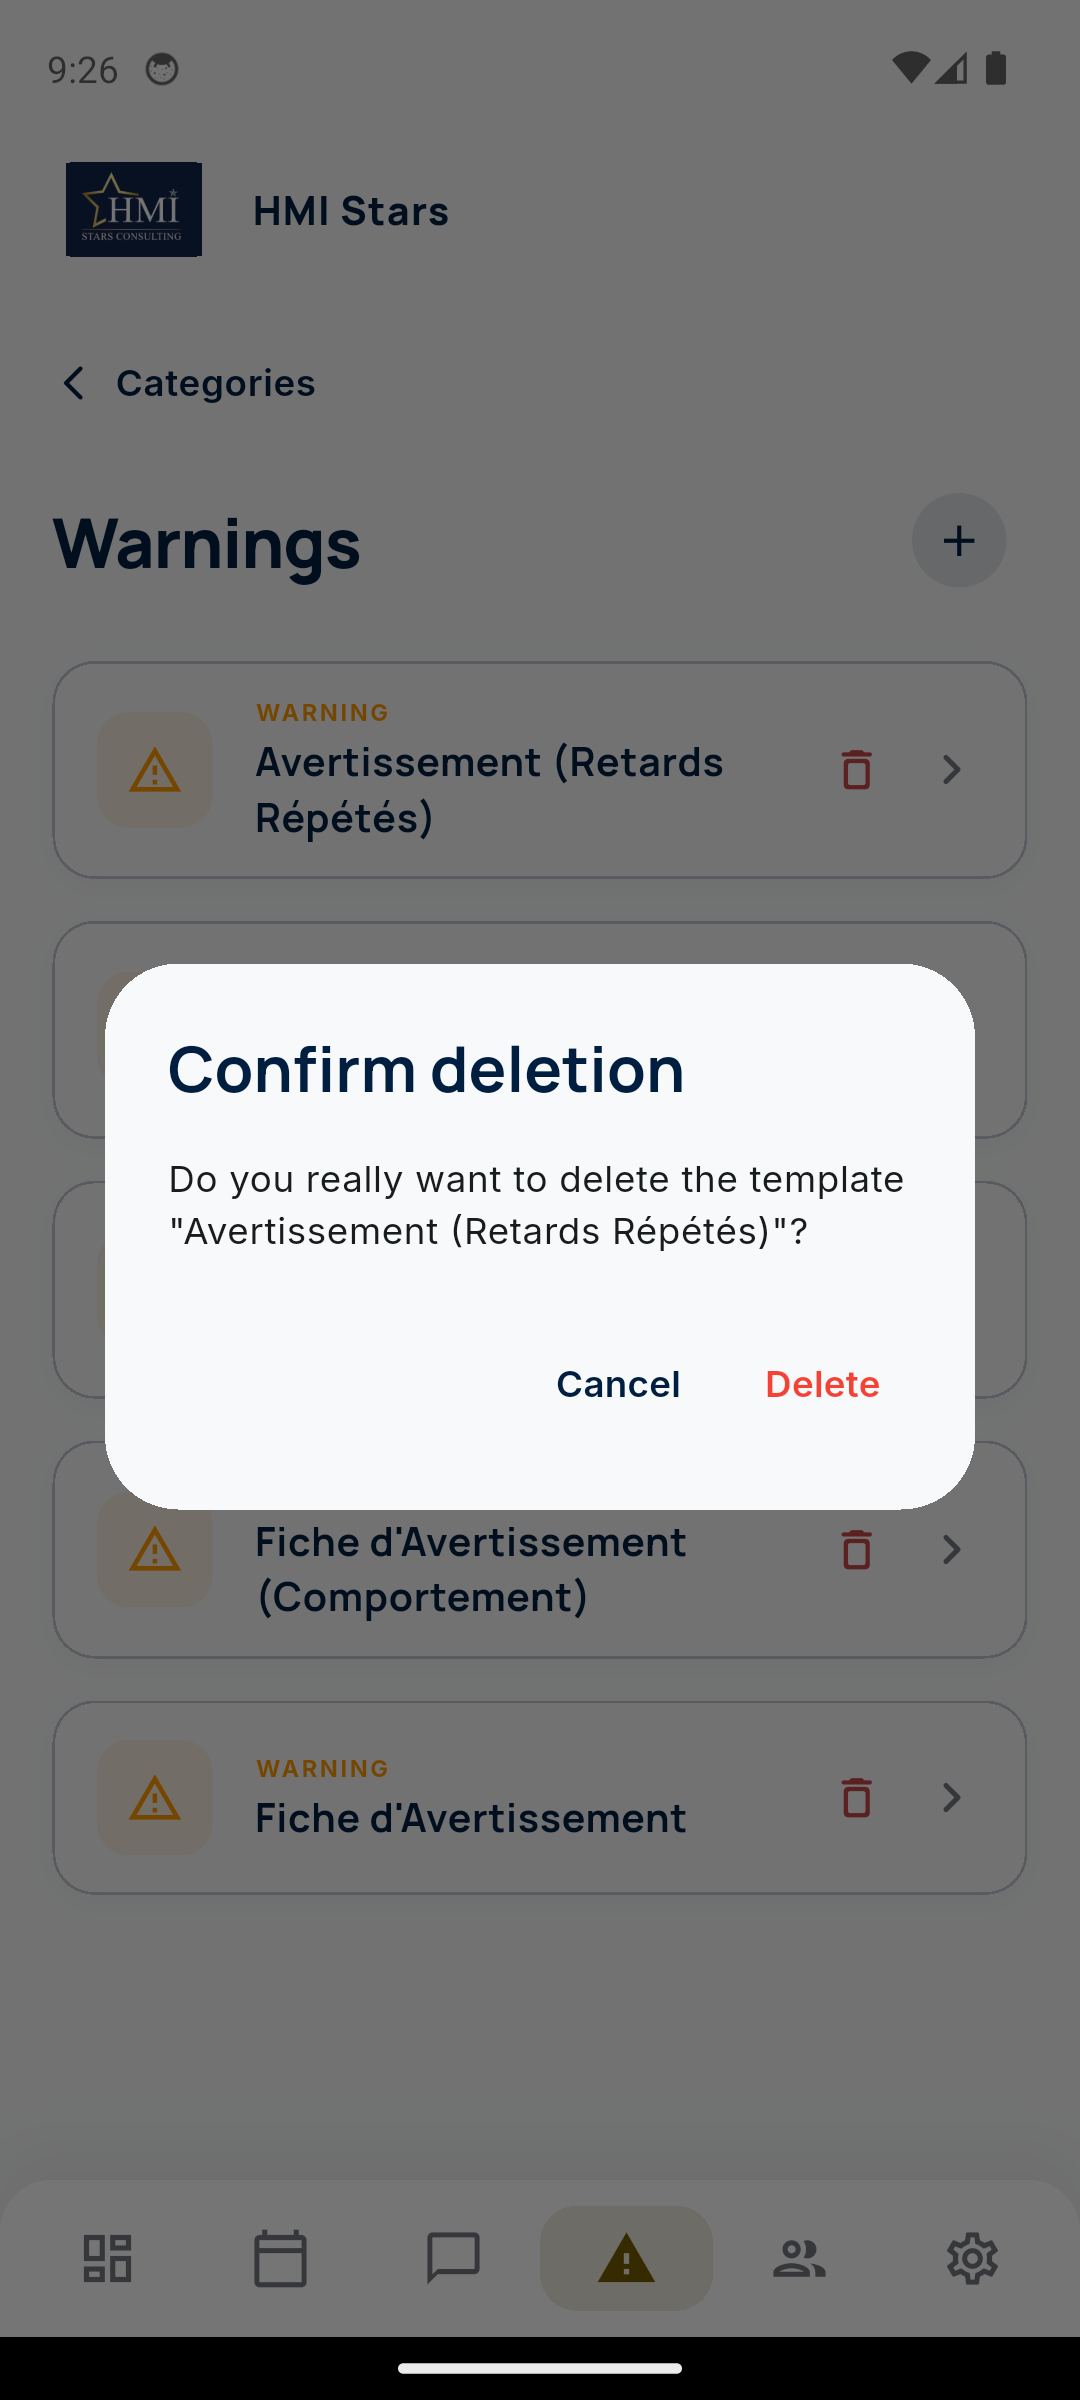
\includegraphics[width=1\textwidth]{project_images/App_light_and_english/delete_av.png}
        \caption{Delete Confirmation}
        \label{fig:m_warn_delete}
    \end{subfigure}
    \caption{Mobile Application - Warning Template Creation and Deletion}
    \label{fig:m_warnings_management}
\end{figure}

\paragraph{Modifying, Viewing, and Sending Warnings}
Once a template is ready, managers can modify its content, preview the letter, select employee recipients, and send the dispatch via Gmail. Figure \ref{fig:m_warnings_send_flow} shows the edit form, the letter preview screen, the recipient selector dialog, and the pre-filled Gmail interface.

\begin{figure}[H]
    \centering
    \begin{subfigure}[b]{0.33\textwidth}
        \centering
        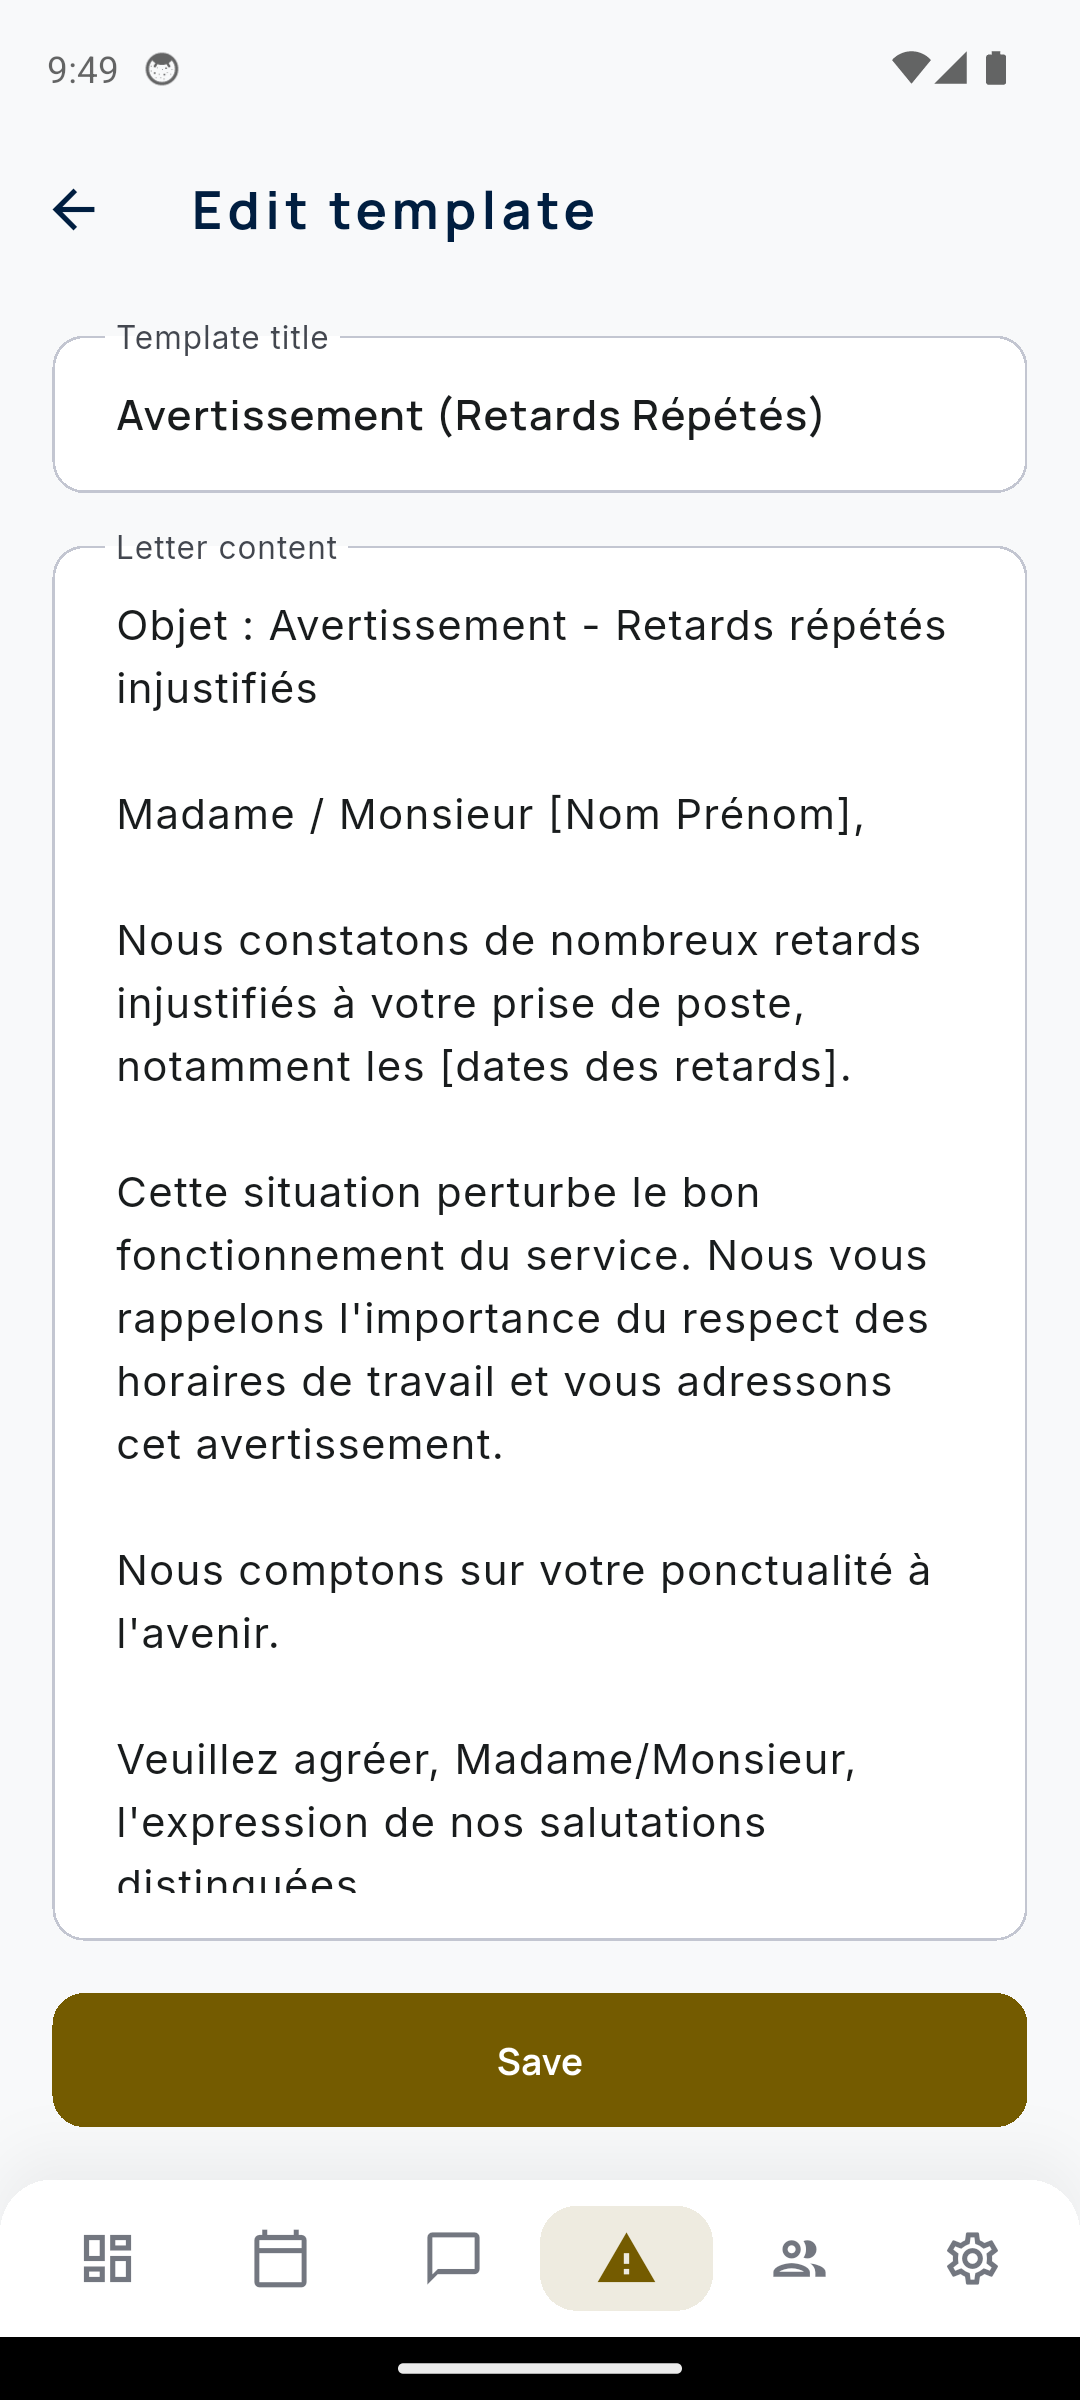
\includegraphics[width=\textwidth]{project_images/App_light_and_english/modify_av.png}
        \caption{Modify Template}
        \label{fig:m_warn_modify}
    \end{subfigure}
    \hfil
    \begin{subfigure}[b]{0.33\textwidth}
        \centering
        
\includegraphics[width=\textwidth]{project_images/App_light_and_english/flutter_19.png}
        \caption{Letter Preview}
        \label{fig:m_warn_preview}
    \end{subfigure}
    \hfil
    \begin{subfigure}[b]{0.33\textwidth}
        \centering
        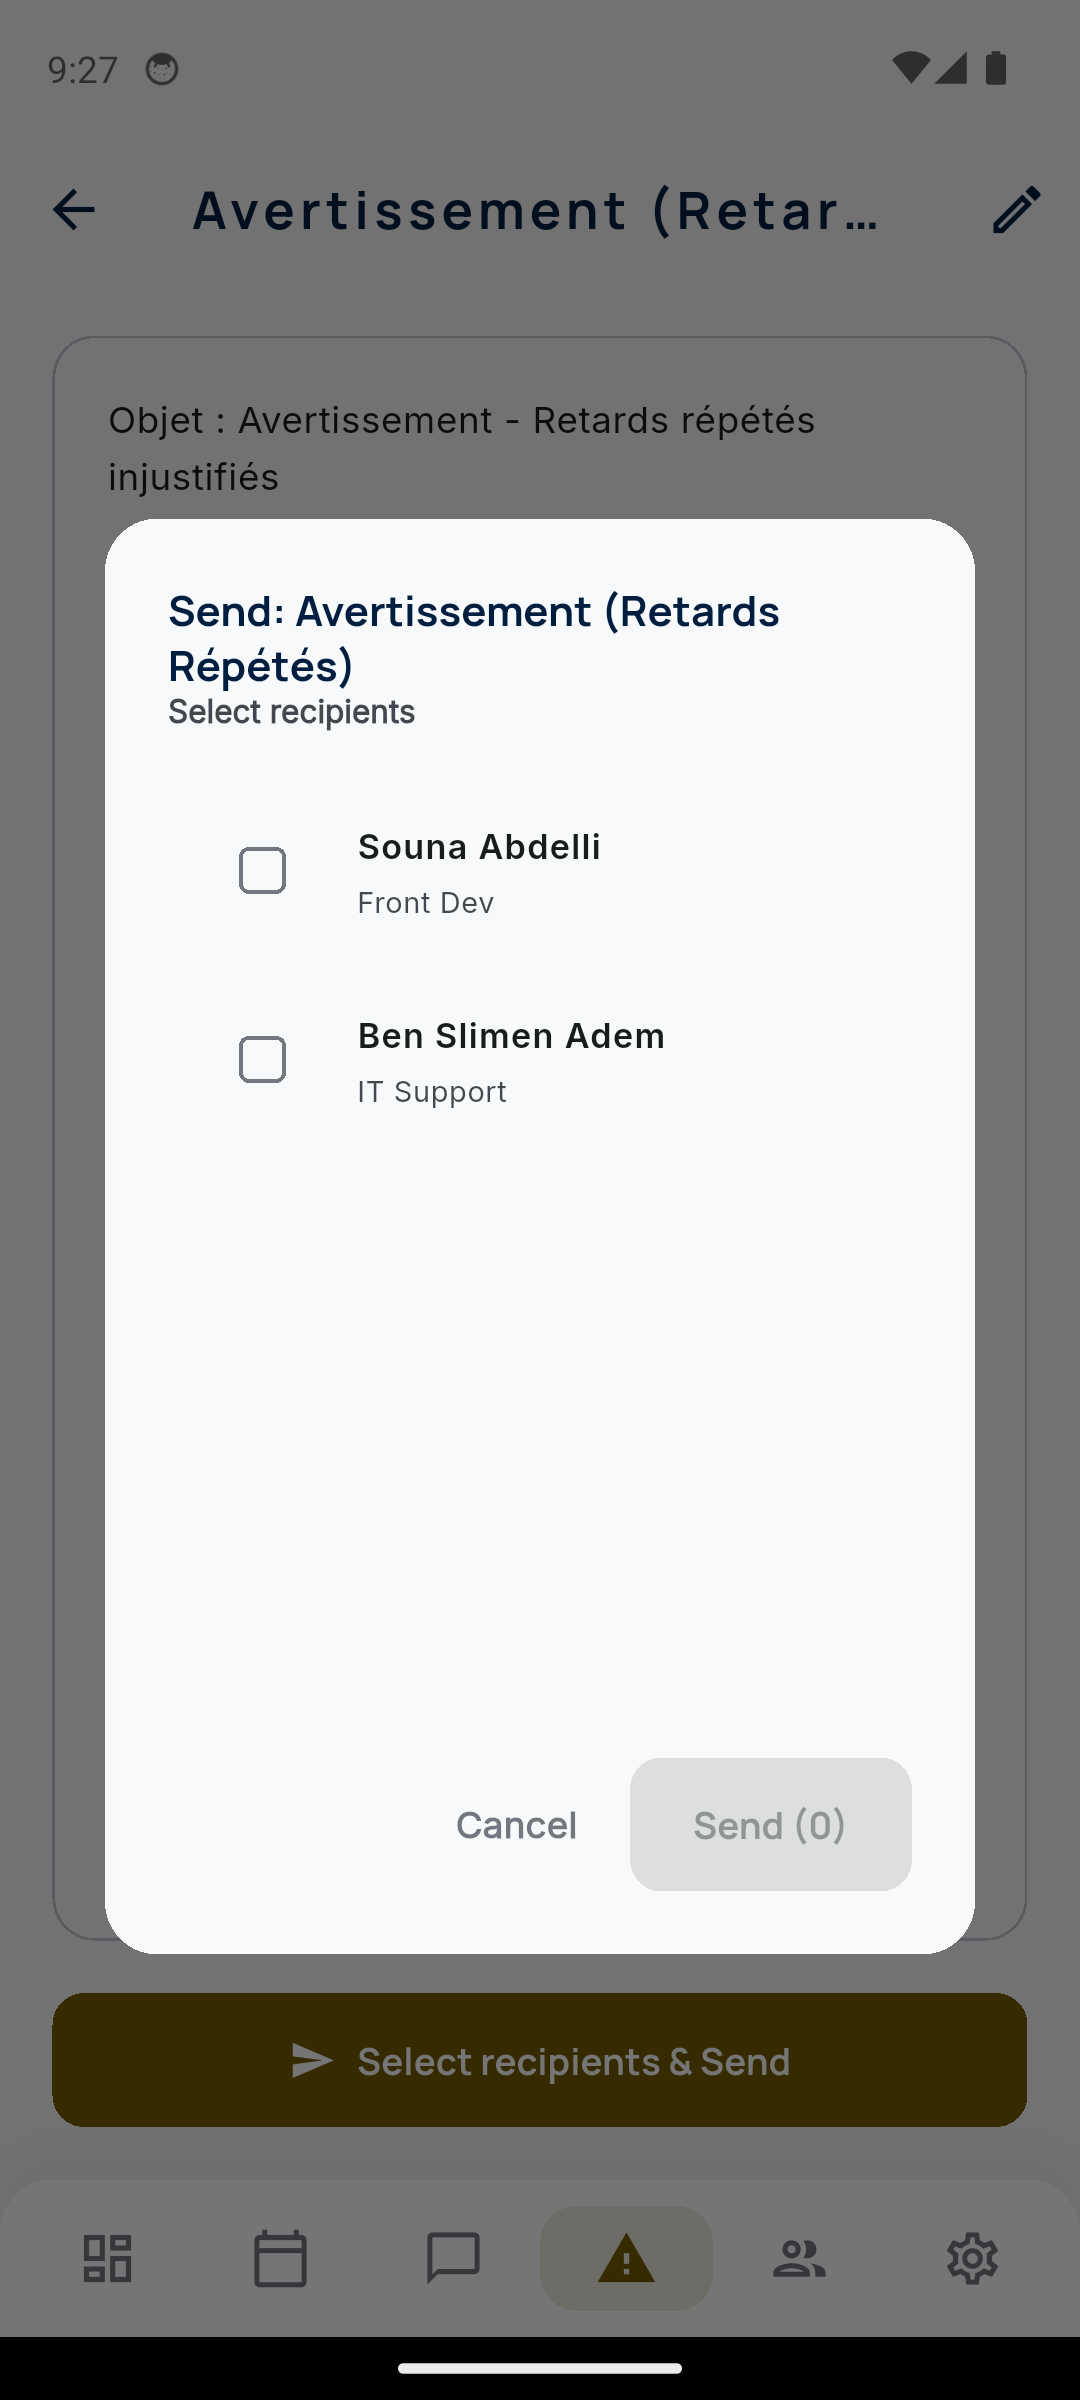
\includegraphics[width=\textwidth]{project_images/App_light_and_english/send_av.png}
        \caption{Recipient Selector}
        \label{fig:m_warn_select_recipients}
    \end{subfigure}
    \hfil
    \begin{subfigure}[b]{0.33\textwidth}
        \centering
        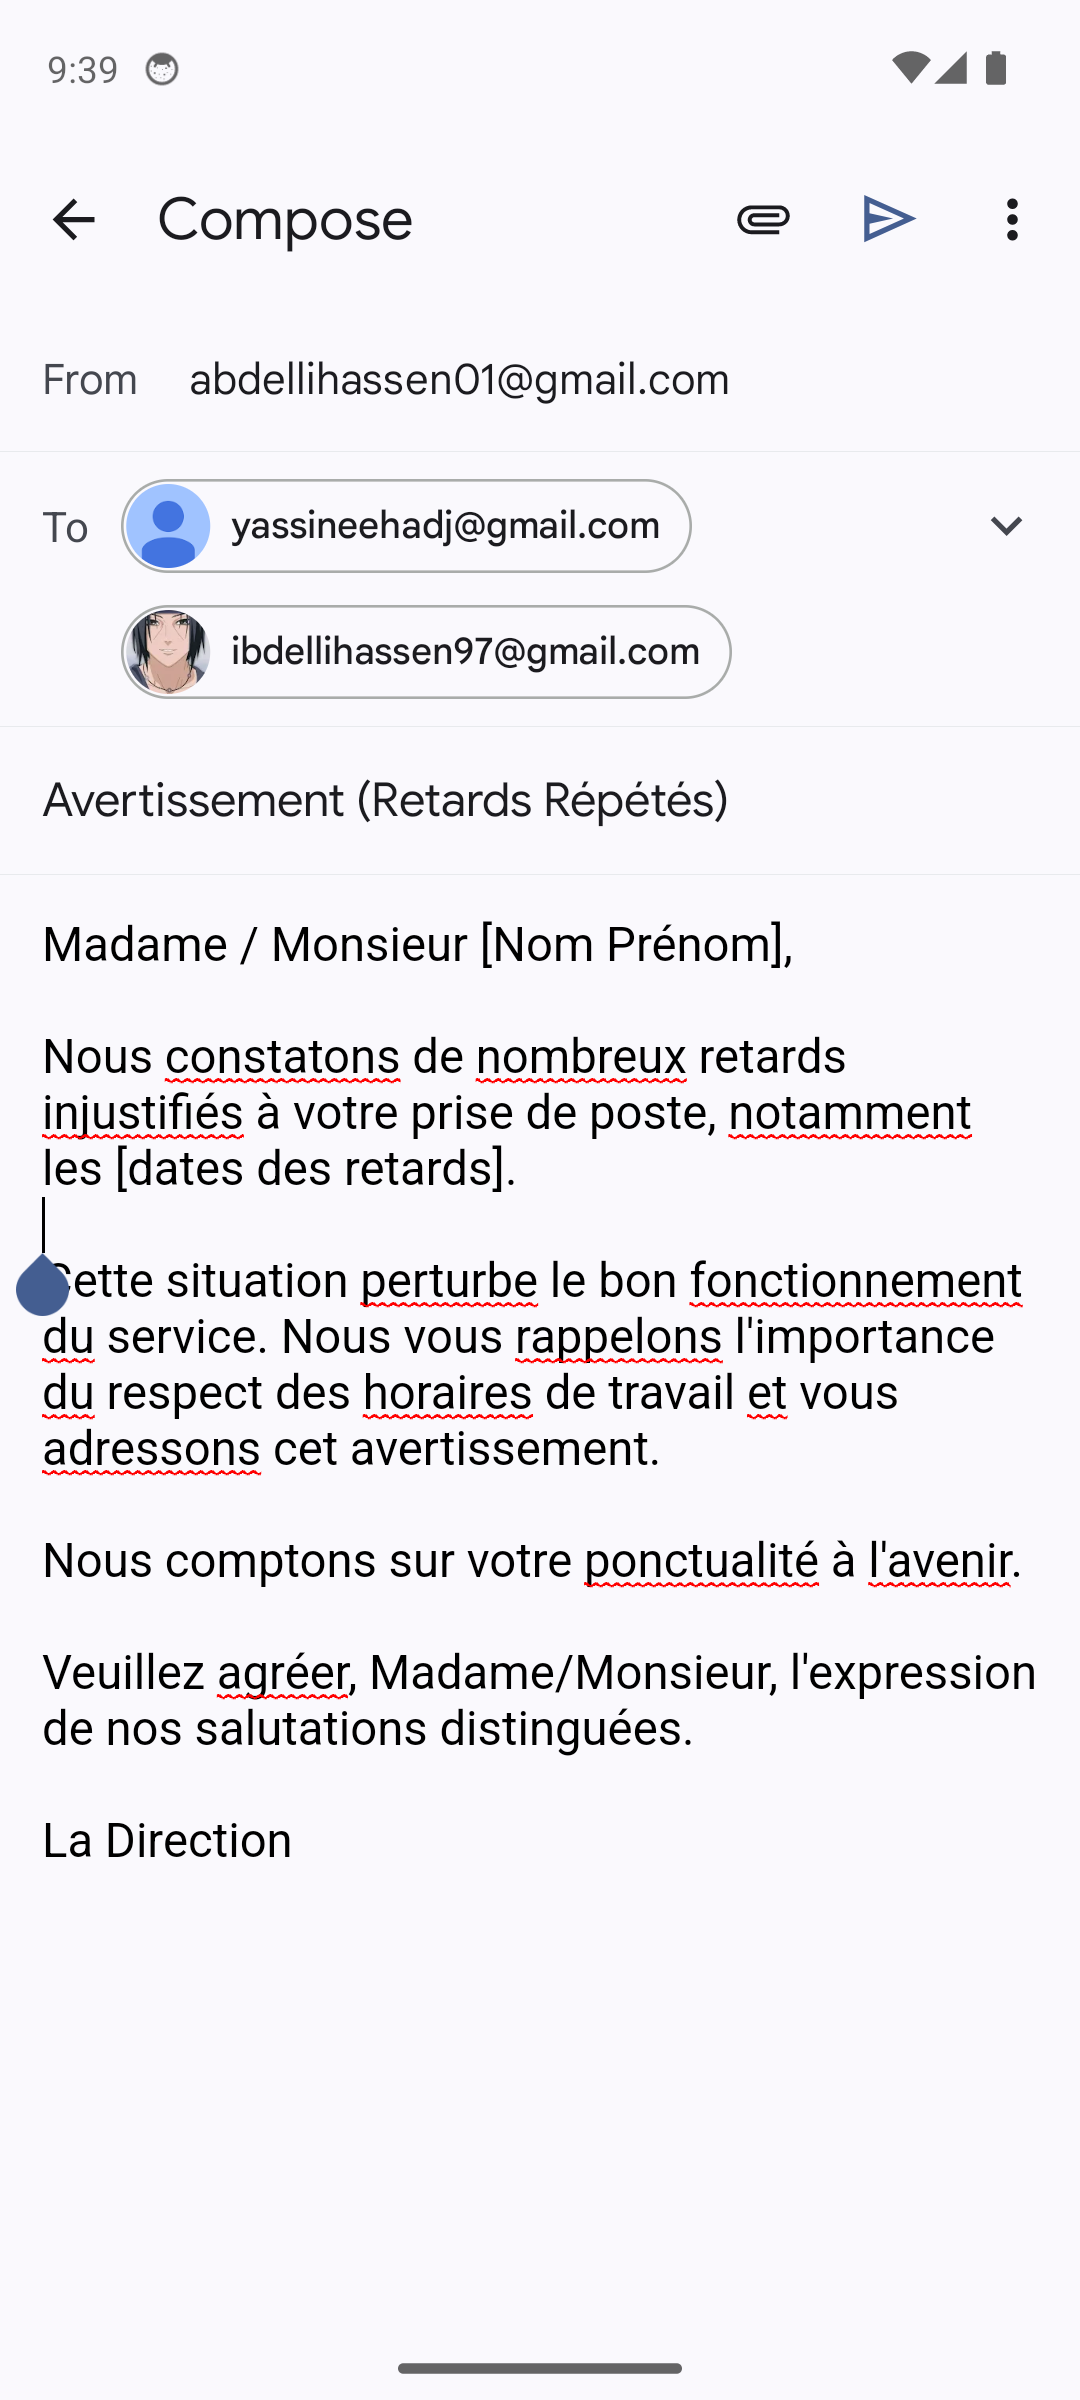
\includegraphics[width=\textwidth]{project_images/App_light_and_english/mail_av.png}
        \caption{Gmail Redirect}
        \label{fig:m_warn_gmail}
    \end{subfigure}
    \caption{Modifying, Viewing, Selecting Recipients, and Sending Warnings}
    \label{fig:m_warnings_send_flow}
\end{figure}

\paragraph{App Settings and Configurations}
Finally, the settings view (Figure \ref{fig:m_settings_flow}) allows users to modify profile parameters, toggle languages (FR/EN) and themes (Light/Dark), and update corporate legal structures.

\begin{figure}[H]
    \centering
    \begin{subfigure}[b]{0.48\textwidth}
        \centering
        
\includegraphics[width=1\textwidth]{project_images/App_light_and_english/flutter_26.png}
        \caption{Account Preferences}
    \end{subfigure}
    \begin{subfigure}[b]{0.48\textwidth}
        \centering
        
\includegraphics[width=1\textwidth]{project_images/App_light_and_english/flutter_27.png}
        \caption{Company Corporate Data}
    \end{subfigure}
    \caption{Mobile Application - Settings and Personalization Interfaces}
    \label{fig:m_settings_flow}
\end{figure}

\paragraph{Mobile Application Dark Mode Theme Options}
To ensure high usability under low-light environments and satisfy user preferences, the mobile application supports a fully integrated Dark Mode theme option. Figure \ref{fig:mobile_dark_mode} illustrates the login interface, main dashboard, and settings screens rendered in Dark Mode.

\begin{figure}[H]
    \centering
    \begin{subfigure}[b]{0.32\textwidth}
        \centering
        
\includegraphics[width=\textwidth]{project_images/App_dark_and_french/flutter_01.png}
        \caption{Login Screen}
        \label{fig:m_dark_login}
    \end{subfigure}
    \hfill
    \begin{subfigure}[b]{0.32\textwidth}
        \centering
        
\includegraphics[width=\textwidth]{project_images/App_dark_and_french/flutter_03.png}
        \caption{Dashboard Overview}
        \label{fig:m_dark_dashboard}
    \end{subfigure}
    \hfill
    \begin{subfigure}[b]{0.32\textwidth}
        \centering
        
\includegraphics[width=\textwidth]{project_images/App_dark_and_french/flutter_26.png}
        \caption{Settings Screen}
        \label{fig:m_dark_settings}
    \end{subfigure}
    \caption{Mobile Application - Dark Mode Theme Interfaces}
    \label{fig:mobile_dark_mode}
\end{figure}



\subsubsection{Web Application Interfaces}
The web application provides a comprehensive administrative interface for HMI Stars managers. It is presented in order of the web platform's navigation flow.

\paragraph{Authentication, Password Recovery, and OTP Flow}
Figure \ref{fig:web_auth_flow} shows the authentication system. It includes the Login page, Password Recovery requests, verification OTP codes, current password validations.

\begin{figure}[H]
    \centering
    \begin{subfigure}[b]{0.80\textwidth}
        \centering
        
\includegraphics[width=\textwidth]{project_images/Plat_light_and_french/flutter_01_1.png}
        \caption{Login Interface}
    \end{subfigure}
    
    \vspace{0.3cm}
    
    \begin{subfigure}[b]{0.80\textwidth}
        \centering
        
\includegraphics[width=\textwidth]{project_images/Plat_light_and_french/flutter_02_1.png}
        \caption{Password Recovery Form}
    \end{subfigure}
    
    \vspace{0.3cm}
    
    \begin{subfigure}[b]{0.80\textwidth}
        \centering
        
\includegraphics[width=\textwidth]{project_images/Plat_light_and_french/flutter_03_1.png}
        \caption{OTP Recovery Dialogue}
    \end{subfigure}
    \caption{Web Platform - Authentication, Recovery, and OTP Dialogs}
    \label{fig:web_auth_flow}
\end{figure}

\paragraph{Platform Dashboard}
The dashboard displays aggregated charts representing key metrics such as employee counts, leave request ratios, and active companies, as shown in Figure \ref{fig:w_dash}.

\begin{figure}[H]
    \centering
    
\includegraphics[width=1\textwidth]{project_images/Plat_light_and_french/flutter_01.png}
    \caption{Dashboard Interface}
    \label{fig:w_dash}
\end{figure}

\paragraph{Client Companies Directory}
Managers browse client portfolios using the Company Directory grid, as shown in Figure \ref{fig:web_companies_directory}. They can also create and register new enterprises using the registration form, as illustrated in Figure \ref{fig:web_company_creation}.

\begin{figure}[H]
    \centering
    
\includegraphics[width=1\textwidth]{project_images/Plat_light_and_french/flutter_02.png}
    \caption{Web Platform - Client Companies Directory}
    \label{fig:web_companies_directory}
\end{figure}

\begin{figure}[H]
    \centering
    
\includegraphics[width=1\textwidth]{project_images/Plat_light_and_french/flutter_04.png}
    \caption{Web Platform - Company Registration Form}
    \label{fig:web_company_creation}
\end{figure}

\paragraph{Company Detailed Workspace Tab System}
Clicking on a company card opens its detailed workspace, which is organized into five tabs. Figure \ref{fig:web_company_workspace} shows the details panel, while Figure \ref{fig:web_company_modifier} presents its edit form.

\begin{figure}[H]
    \centering
    
\includegraphics[width=1\textwidth]{project_images/Plat_light_and_french/flutter_06.png}
    \caption{Web Platform - Detailed Company Workspace}
    \label{fig:web_company_workspace}
\end{figure}

\begin{figure}[H]
    \centering
    
\includegraphics[width=1\textwidth]{project_images/Plat_light_and_french/flutter_31.png}
    \caption{Web Platform - Company Information Modifier Form}
    \label{fig:web_company_modifier}
\end{figure}

\paragraph{Company Employees Tab \& Registry}
The Employees tab manages active contracts, displaying a comprehensive list of all employees within the selected company (Figure \ref{fig:web_employee_registry}). From this registry interface, managers can see detailed profiles, archive or delete records, or access individual employee cards (Figure \ref{fig:web_profile_card}). Clicking on the details button allows managers to inspect the complete record, while the modify button enables direct edits to the employee's contract and personal data.

\begin{figure}[H]
    \centering
    
\includegraphics[width=1\textwidth]{project_images/Plat_light_and_french/flutter_07.png}
    \caption{Web Platform - Active Employee Registry}
    \label{fig:web_employee_registry}
\end{figure}

\begin{figure}[H]
    \centering
    
\includegraphics[width=1\textwidth]{project_images/Plat_light_and_french/flutter_13.png}
    \caption{Web Platform - Detailed Profile Card}
    \label{fig:web_profile_card}
\end{figure}

\paragraph{Employee Creation \& Detailed Inspector Dialogs}
Registering new staff is handled via a dedicated creation form (Figure \ref{fig:web_new_employee_form}) that captures personal information and contract parameters. Once created, detailed records can be inspected dynamically through an overlay panel (Figure \ref{fig:web_employee_details_dialog}) which aggregates contract logs and personal details.

\begin{figure}[H]
    \centering
    
\includegraphics[width=1\textwidth]{project_images/Plat_light_and_french/flutter_12.png}
    \caption{Web Platform - New Employee Registration Form}
    \label{fig:web_new_employee_form}
\end{figure}

\begin{figure}[H]
    \vspace{1cm}
    \centering
    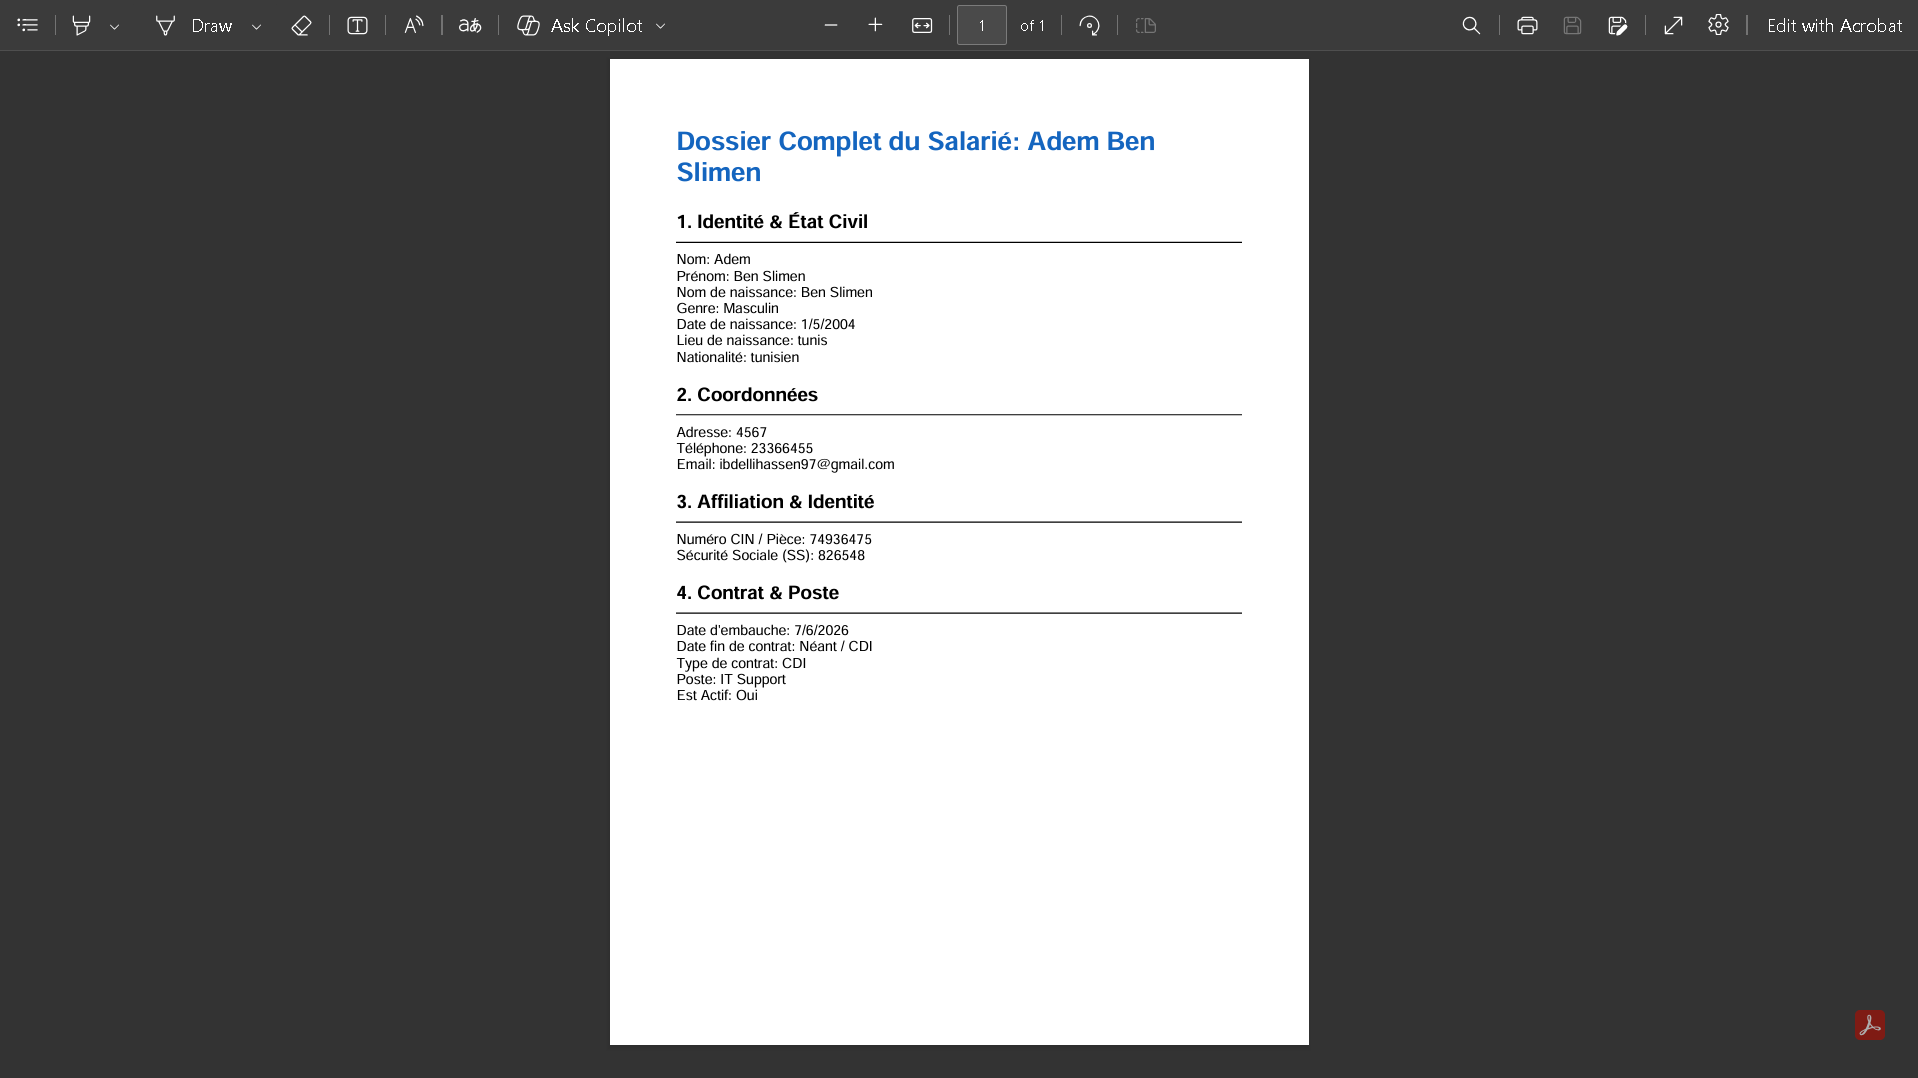
\includegraphics[width=1\textwidth]{project_images/employee_data_fr.png}
    \caption{Web Platform - Employee Details Dialog}
    \label{fig:web_employee_details_dialog}
\end{figure}

\paragraph{Bilingual Attendance Export}
Managers can export the registry's lists or retrieve specific attendance tracking sheets for any given month in a fully bilingual layout (French and English) using the attendance export utility dialog (Figure \ref{fig:web_attendance_export_dialog}). This allows administrative personnel to download spreadsheets structured for local payroll systems.

\begin{figure}[H]
    \centering
    
\includegraphics[width=1\textwidth]{project_images/Plat_light_and_french/flutter_15.png}
    \caption{Web Platform - Attendance Export Dialog}
    \label{fig:web_attendance_export_dialog}
\end{figure}

\paragraph{Company Employee Archives Tab}
The Employee Archives tab retains records of departing or terminated employees, as illustrated in Figure \ref{fig:web_archives_tab}.

\begin{figure}[H]
    \centering
    
\includegraphics[width=0.9\textwidth]{project_images/Plat_light_and_french/flutter_08.png}
    \caption{Web Platform - Workspace Employee Archives Tab}
    \label{fig:web_archives_tab}
\end{figure}

\paragraph{Company Warnings Tab}
The Warnings tab manages legal warning dispatches and default templates. Managers can browse warning categories, pre-made legal notices, and dispatch records from the main warnings workspace dashboard (Figure \ref{fig:web_warnings_workspace}).

\begin{figure}[H]
    \centering
    
\includegraphics[width=1\textwidth]{project_images/Plat_light_and_french/flutter_09.png}
    \caption{Web Platform - Warnings Workspace Dashboard}
    \label{fig:web_warnings_workspace}
\end{figure}

\paragraph{Custom Template Editor}
Administrators can customize or create new warning dispatches using the interactive template builder form (Figure \ref{fig:web_warnings_editor}), which allows direct editing of the letter content.

\begin{figure}[H]
    \centering
    
\includegraphics[width=1\textwidth]{project_images/Plat_light_and_french/flutter_21.png}
    \caption{Web Platform - Warnings Custom Editor Form}
    \label{fig:web_warnings_editor}
\end{figure}

\paragraph{Recipient Selection \& Dispatch Preview}
Once the letter is ready, managers select recipients using a search-enabled recipient list dialog (Figure \ref{fig:web_warnings_recipient}). Before dispatching the notice, the system displays a live layout visualization of the generated email letter (Figure \ref{fig:web_warnings_preview}) to verify formatting.

\begin{figure}[H]
    \centering
    
\includegraphics[width=1\textwidth]{project_images/Plat_light_and_french/flutter_22.png}
    \caption{Web Platform - Warnings Recipient Selector Dialog}
    \label{fig:web_warnings_recipient}
\end{figure}

\begin{figure}[H]
    \centering
    
\includegraphics[width=1\textwidth]{project_images/Plat_light_and_french/flutter_24.png}
    \caption{Web Platform - Warnings Email Letter Preview}
    \label{fig:web_warnings_preview}
\end{figure}

\paragraph{Company Notes and Reminders Tab}
The Notes \& Reminders tab allows consultants to log internal notes. Figure \ref{fig:web_notes_flow} shows the notes board and the note creation dialog.

\begin{figure}[H]
    \centering
    \begin{subfigure}[b]{0.85\textwidth}
        \centering
        
\includegraphics[width=\textwidth]{project_images/Plat_light_and_french/flutter_13.png}
        \caption{Company Notes Board}
    \end{subfigure}
    
    \vspace{0.3cm}
    
    \begin{subfigure}[b]{0.85\textwidth}
        \centering
        
\includegraphics[width=\textwidth]{project_images/Plat_light_and_french/flutter_14.png}
        \caption{Add Note Dialog}
    \end{subfigure}
    \caption{Web Platform - Workspace Notes and Reminders Tab}
    \label{fig:web_notes_flow}
\end{figure}

\paragraph{Interactive Leave Request Supervision}
Leave requests are managed through a validation dashboard. Figure \ref{fig:web_leaves_supervision} shows the requests list and the details modal.

\begin{figure}[H]
    \centering
    \begin{subfigure}[b]{0.85\textwidth}
        \centering
        
\includegraphics[width=\textwidth]{project_images/Plat_light_and_french/flutter_18.png}
        \caption{Leave Requests Dashboard}
    \end{subfigure}
    
    \vspace{0.3cm}
    
    \begin{subfigure}[b]{0.85\textwidth}
        \centering
        
\includegraphics[width=\textwidth]{project_images/Plat_light_and_french/flutter_19.png}
        \caption{Leave Details Panel}
    \end{subfigure}
    \caption{Web Platform - Leaves and Absences Supervision Panel}
    \label{fig:web_leaves_supervision}
\end{figure}

\paragraph{Central Messaging Workspace}
The support messaging panel manages real-time interactions with client managers, including the chat interface and the shared document previews, as shown in Figure \ref{fig:web_messaging_workspace}.

\begin{figure}[H]
    \centering
    \begin{subfigure}[b]{0.85\textwidth}
        \centering
        
\includegraphics[width=\textwidth]{project_images/Plat_light_and_french/flutter_06.png}
        \caption{Support Messaging Channel}
    \end{subfigure}
    
    \vspace{0.3cm}
    
    \begin{subfigure}[b]{0.85\textwidth}
        \centering
        
\includegraphics[width=\textwidth]{project_images/Plat_light_and_french/flutter_07.png}
        \caption{Shared Files Directory}
    \end{subfigure}
    \caption{Web Platform - Real-time Messagerie Workspace}
    \label{fig:web_messaging_workspace}
\end{figure}

\paragraph{HR Document Previewer}
The platform includes an internal PDF previewer for files like KBIS extracts, VAT forms, and RIBs, as displayed in Figure \ref{fig:web_pdf_preview}.

\begin{figure}[H]
    \centering
    
\includegraphics[width=0.9\textwidth]{project_images/Plat_light_and_french/flutter_20.png}
    \caption{Web Platform - HR Document PDF Preview Dialog}
    \label{fig:web_pdf_preview}
\end{figure}

\paragraph{General Supervision Calendar}
A consolidated calendar view helps administrators track attendance across all client companies, as shown in Figure \ref{fig:web_general_calendar}.

\begin{figure}[H]
    \centering
    
\includegraphics[width=0.9\textwidth]{project_images/Plat_light_and_french/flutter_27.png}
    \caption{Web Platform - General Supervision Attendance Calendar}
    \label{fig:web_general_calendar}
\end{figure}

\paragraph{Settings, User Accounts, and Platform Admin Listings}
Figure \ref{fig:web_config_flow} shows the platform configuration tools, including the settings page, the platform admin list, and the user invitation dialog.

\begin{figure}[H]
    \centering
    \begin{subfigure}[b]{0.85\textwidth}
        \centering
        
\includegraphics[width=\textwidth]{project_images/Plat_light_and_french/flutter_15.png}
        \caption{Preferences settings}
    \end{subfigure}
    
    \vspace{0.3cm}
    
    \begin{subfigure}[b]{0.85\textwidth}
        \centering
        
\includegraphics[width=\textwidth]{project_images/Plat_light_and_french/flutter_16.png}
        \caption{Platform Admin Accounts}
    \end{subfigure}
    
    \vspace{0.3cm}
    
    \begin{subfigure}[b]{0.85\textwidth}
        \centering
        
\includegraphics[width=\textwidth]{project_images/Plat_light_and_french/flutter_17.png}
        \caption{Invitation / Edit Dialog}
    \end{subfigure}
    \caption{Web Platform - Settings and Accounts Configurations}
    \label{fig:web_config_flow}
\end{figure}

\paragraph{Web Platform Dark Mode Theme Options}
Similar to the mobile client, the web administration platform supports an alternative Dark Mode theme to reduce eye strain and provide a premium, modern aesthetic for administrative staff. Figure \ref{fig:web_dark_mode} shows the web login page, main analytical dashboard, and preferences configuration screen rendered in Dark Mode.

\begin{figure}[H]
    \centering
    \begin{subfigure}[b]{0.85\textwidth}
        \centering
        
\includegraphics[width=\textwidth]{project_images/Plat_night_and_english/flutter_01.png}
        \caption{Login Interface}
        \label{fig:w_dark_login}
    \end{subfigure}
    
    \vspace{0.3cm}
    
    \begin{subfigure}[b]{0.85\textwidth}
        \centering
        
\includegraphics[width=\textwidth]{project_images/Plat_night_and_english/flutter_02.png}
        \caption{Analytical Dashboard}
        \label{fig:w_dark_dash}
    \end{subfigure}
    
    \vspace{0.3cm}
    
    \begin{subfigure}[b]{0.85\textwidth}
        \centering
        
\includegraphics[width=\textwidth]{project_images/Plat_night_and_english/flutter_16.png}
        \caption{Preferences Settings}
        \label{fig:w_dark_settings}
    \end{subfigure}
    \caption{Web Administration Platform - Dark Mode Theme Interfaces}
    \label{fig:web_dark_mode}
\end{figure}


\paragraph{Platform Utilities}
Figure \ref{fig:web_utilities_flow} shows other utilities, including notification centers, toast popups, automatic alert configuration panels, and manager association dialogs.

\begin{figure}[H]
    \centering
    \begin{subfigure}[b]{0.85\textwidth}
        \centering
        
\includegraphics[width=\textwidth]{project_images/Plat_light_and_french/flutter_23.png}
        \caption{Notification Center Drawer}
    \end{subfigure}
    
    \vspace{0.3cm}
    
    \begin{subfigure}[b]{0.85\textwidth}
        \centering
        
\includegraphics[width=\textwidth]{project_images/Plat_light_and_french/flutter_28.png}
        \caption{Standard success Toast}
    \end{subfigure}
    
    \vspace{0.3cm}
    
    \begin{subfigure}[b]{0.85\textwidth}
        \centering
        
\includegraphics[width=\textwidth]{project_images/Plat_light_and_french/flutter_29.png}
        \caption{Automatic alerts setup}
    \end{subfigure}
    
    \vspace{0.3cm}
    
    \begin{subfigure}[b]{0.85\textwidth}
        \centering
        
\includegraphics[width=\textwidth]{project_images/Plat_light_and_french/flutter_30.png}
        \caption{Associate Managers dialogue}
    \end{subfigure}
    \caption{Web Platform - Dynamic Utility Dialogs and Toast feedback}
    \label{fig:web_utilities_flow}
\end{figure}

\paragraph{Consolidated Reports Export}
The platform also supports exporting consolidated Excel activity spreadsheets for accounting and bookkeeping, as shown in Figure \ref{fig:web_consolidated_export}.

\begin{figure}[H]
    \centering
    
\includegraphics[width=0.9\textwidth]{project_images/Plat_light_and_french/flutter_31.png}
    \caption{Web Platform - Consolidated Activity Reports Export Panel}
    \label{fig:web_consolidated_export}
\end{figure}

\subsubsection{Bilingual Email Templates and Notification Subsystem}
The Supabase authentication service sends bilingual responsive HTML templates for transactional emails, as shown in Figure \ref{fig:email_templates}. Each template features both French (at the top) and English (at the bottom) text.

\begin{figure}[H]
\centering
\begin{subfigure}[b]{0.32\textwidth}
    \centering
    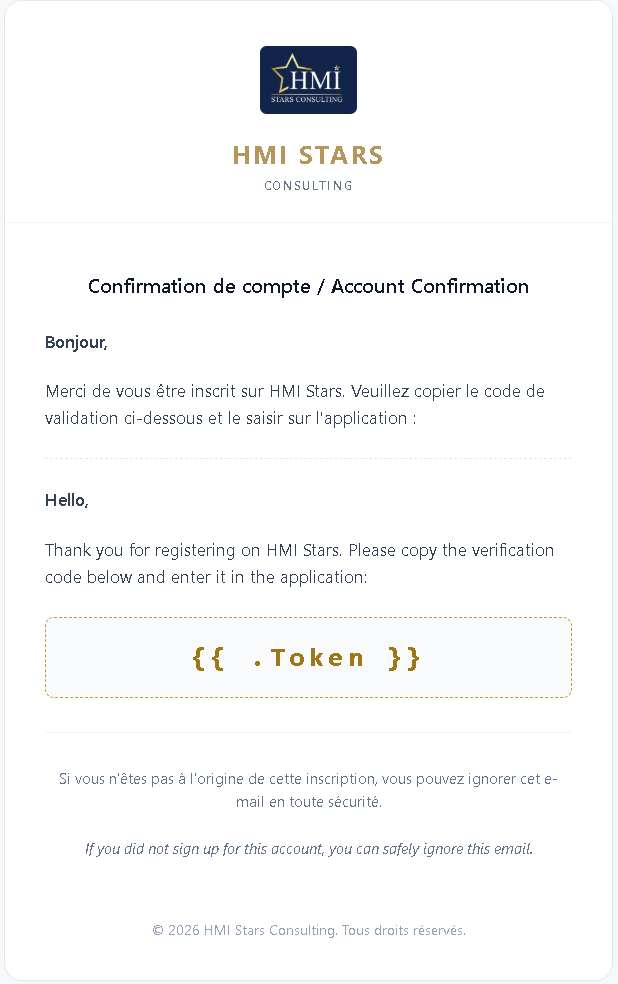
\includegraphics[width=\textwidth]{project_images/mails_preview/confirm_acc_mail.png}
    \caption{Sign Up Confirmation}
\end{subfigure}
\hfill
\begin{subfigure}[b]{0.32\textwidth}
    \centering
    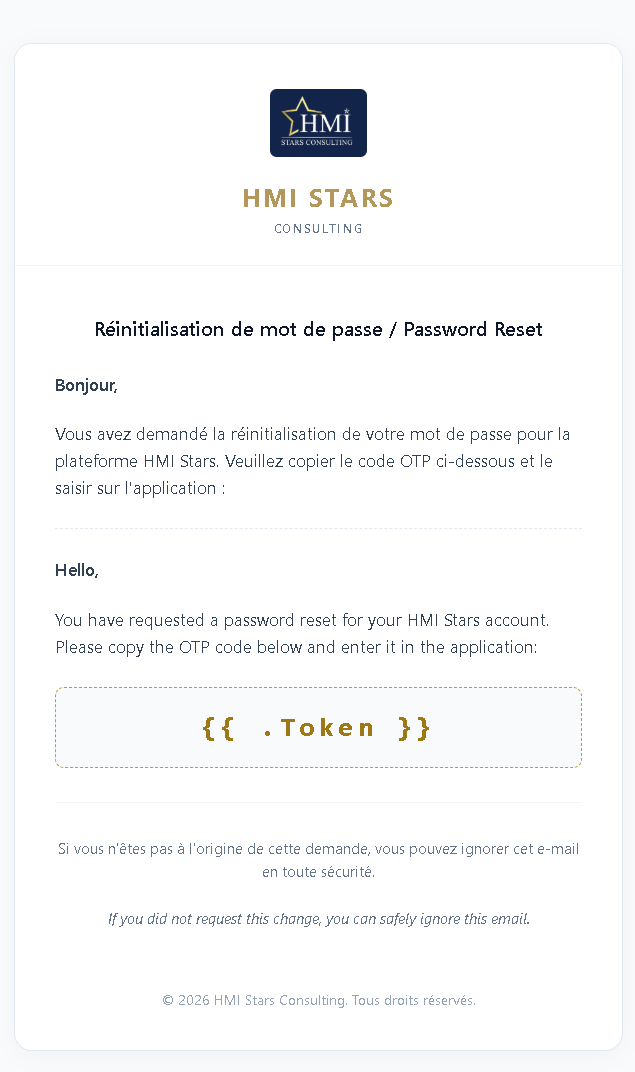
\includegraphics[width=\textwidth]{project_images/mails_preview/password_reset_mail.png}
    \caption{Password Reset OTP}
\end{subfigure}
\hfill
\begin{subfigure}[b]{0.32\textwidth}
    \centering
    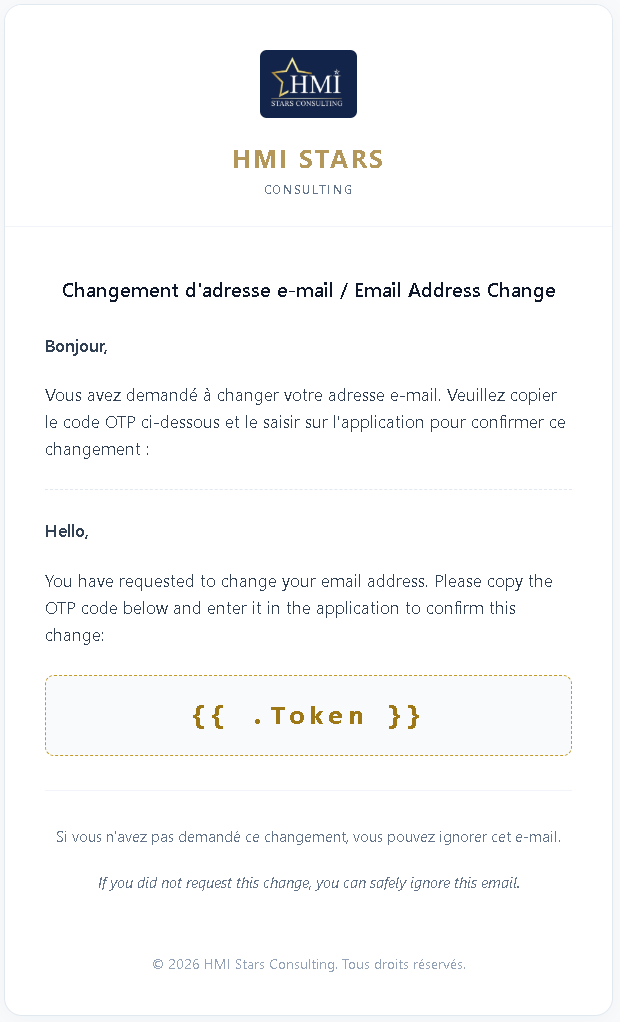
\includegraphics[width=\textwidth]{project_images/mails_preview/mail_otp_change_mail.png}
    \caption{Email Change OTP}
\end{subfigure}

\vspace{0.3cm}

\begin{subfigure}[b]{0.32\textwidth}
    \centering
    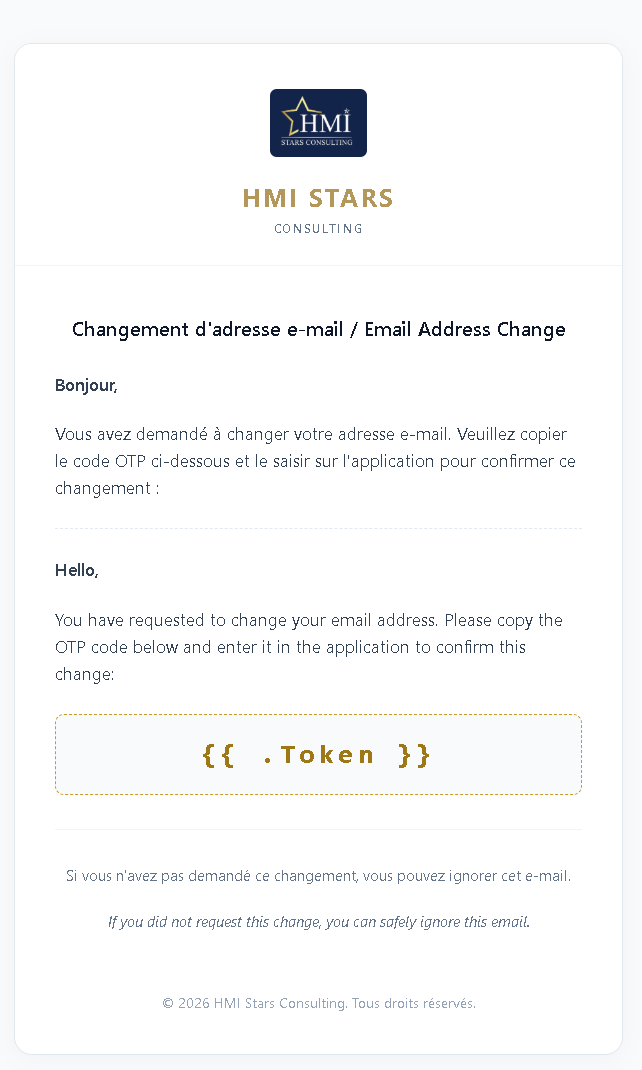
\includegraphics[width=\textwidth]{project_images/mails_preview/mail_change_mail.png}
    \caption{Email Change Confirm}
\end{subfigure}
\hfill
\begin{subfigure}[b]{0.32\textwidth}
    \centering
    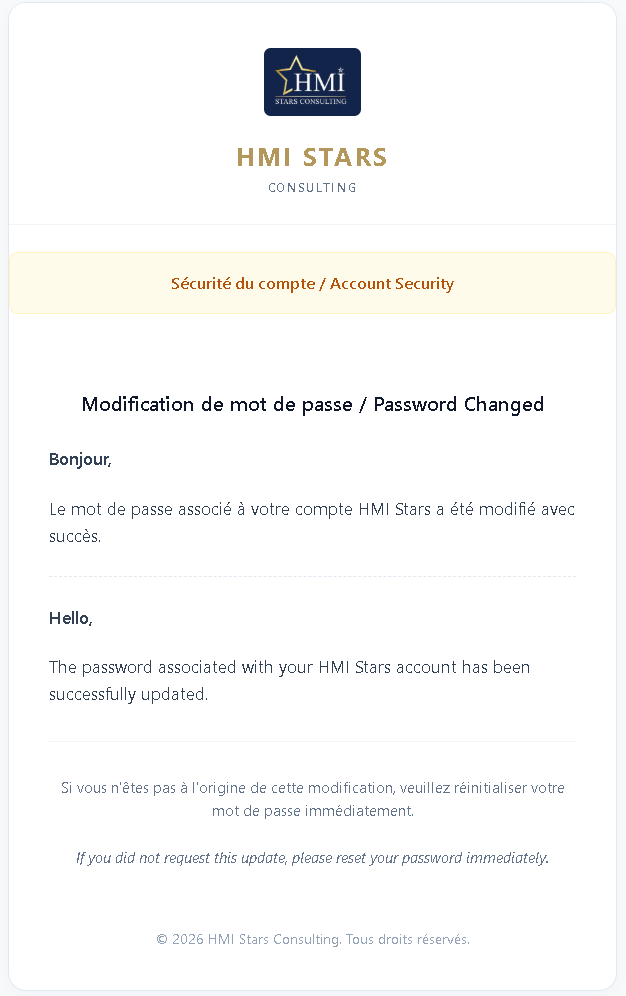
\includegraphics[width=\textwidth]{project_images/mails_preview/pass_change_mail.png}
    \caption{Password Update Notice}
\end{subfigure}
\hfill
\begin{subfigure}[b]{0.32\textwidth}
    \centering
    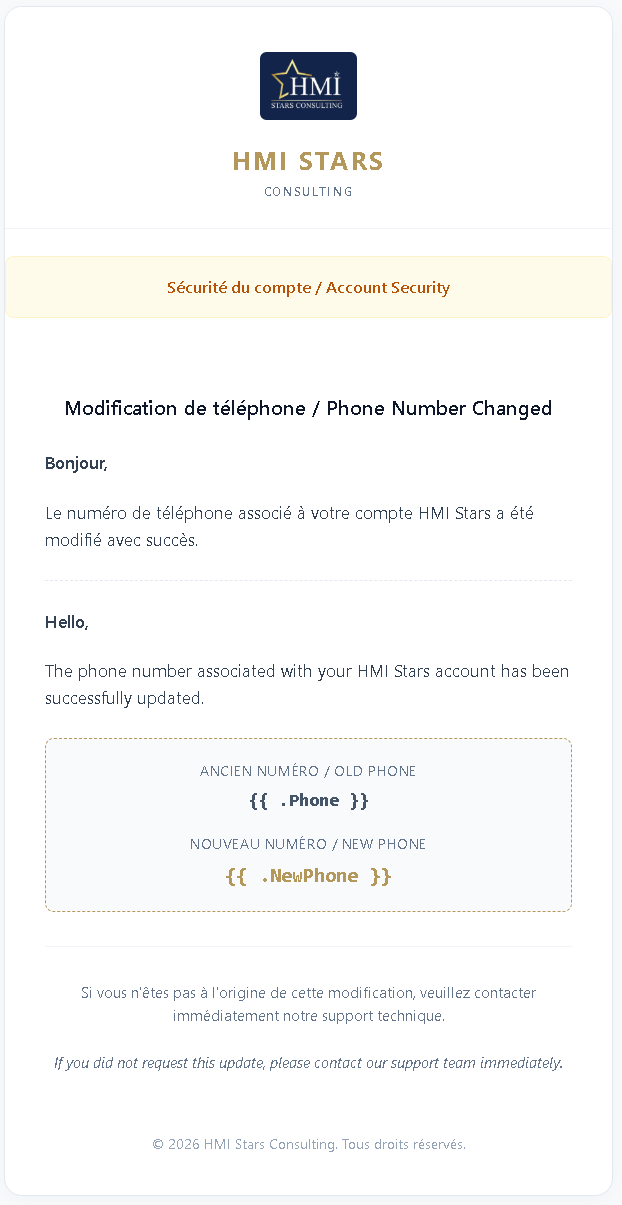
\includegraphics[width=\textwidth]{project_images/mails_preview/nmbr_change_mail.png}
    \caption{Phone Update Notice}
\end{subfigure}
\caption{Supabase Authentication Service - Bilingual Responsive Email Templates}
\label{fig:email_templates}
\end{figure}

In-app alerts are delivered via Firebase Cloud Messaging (FCM), as shown in Figure \ref{fig:fcm_notif_phone}.

\begin{figure}[H]
\centering
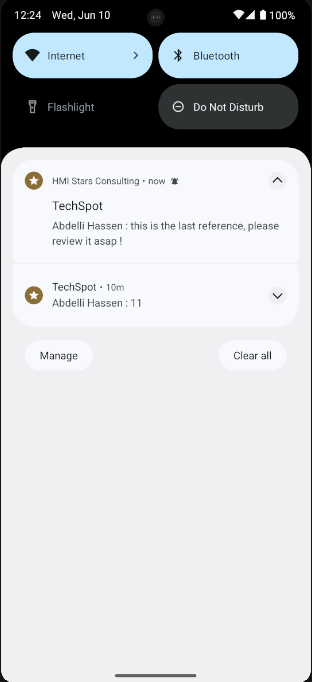
\includegraphics[width=0.45\textwidth]{project_images/phone_notif.png}
\caption{Firebase Cloud Messaging (FCM) Mobile Push Notification}
\label{fig:fcm_notif_phone}
\end{figure}

\subsubsection{Exported Output Demonstrations}
Exported PDF employee files and CSV/Excel attendance files demonstrate the platform's data-generation features, as illustrated in Figure \ref{fig:output_demos}.

\begin{figure}[H]
\centering
\begin{subfigure}[b]{0.48\textwidth}
    \centering
    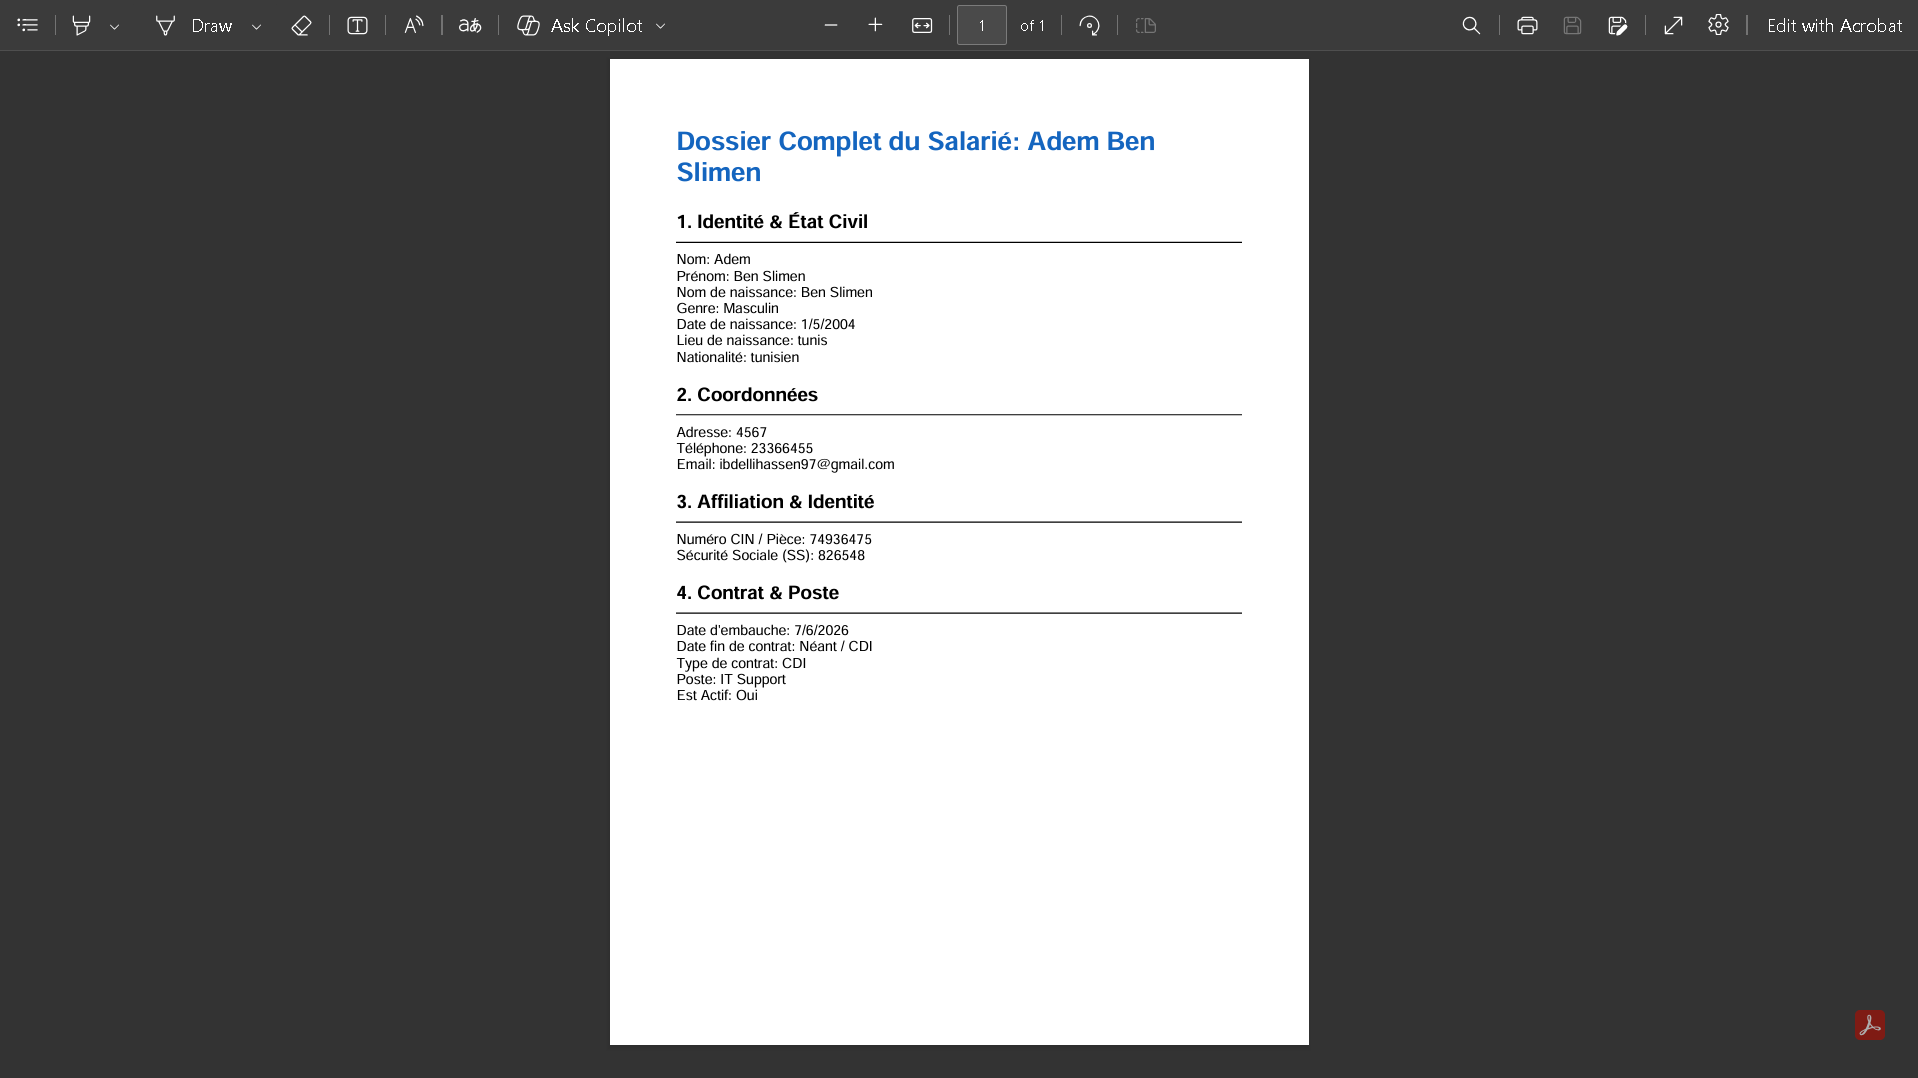
\includegraphics[width=0.85\textwidth]{project_images/employee_data_fr.png}
    \caption{Bilingual PDF Employee File}
    \label{fig:out_pdf}
\end{subfigure}
\hfill
\begin{subfigure}[b]{0.48\textwidth}
    \centering
    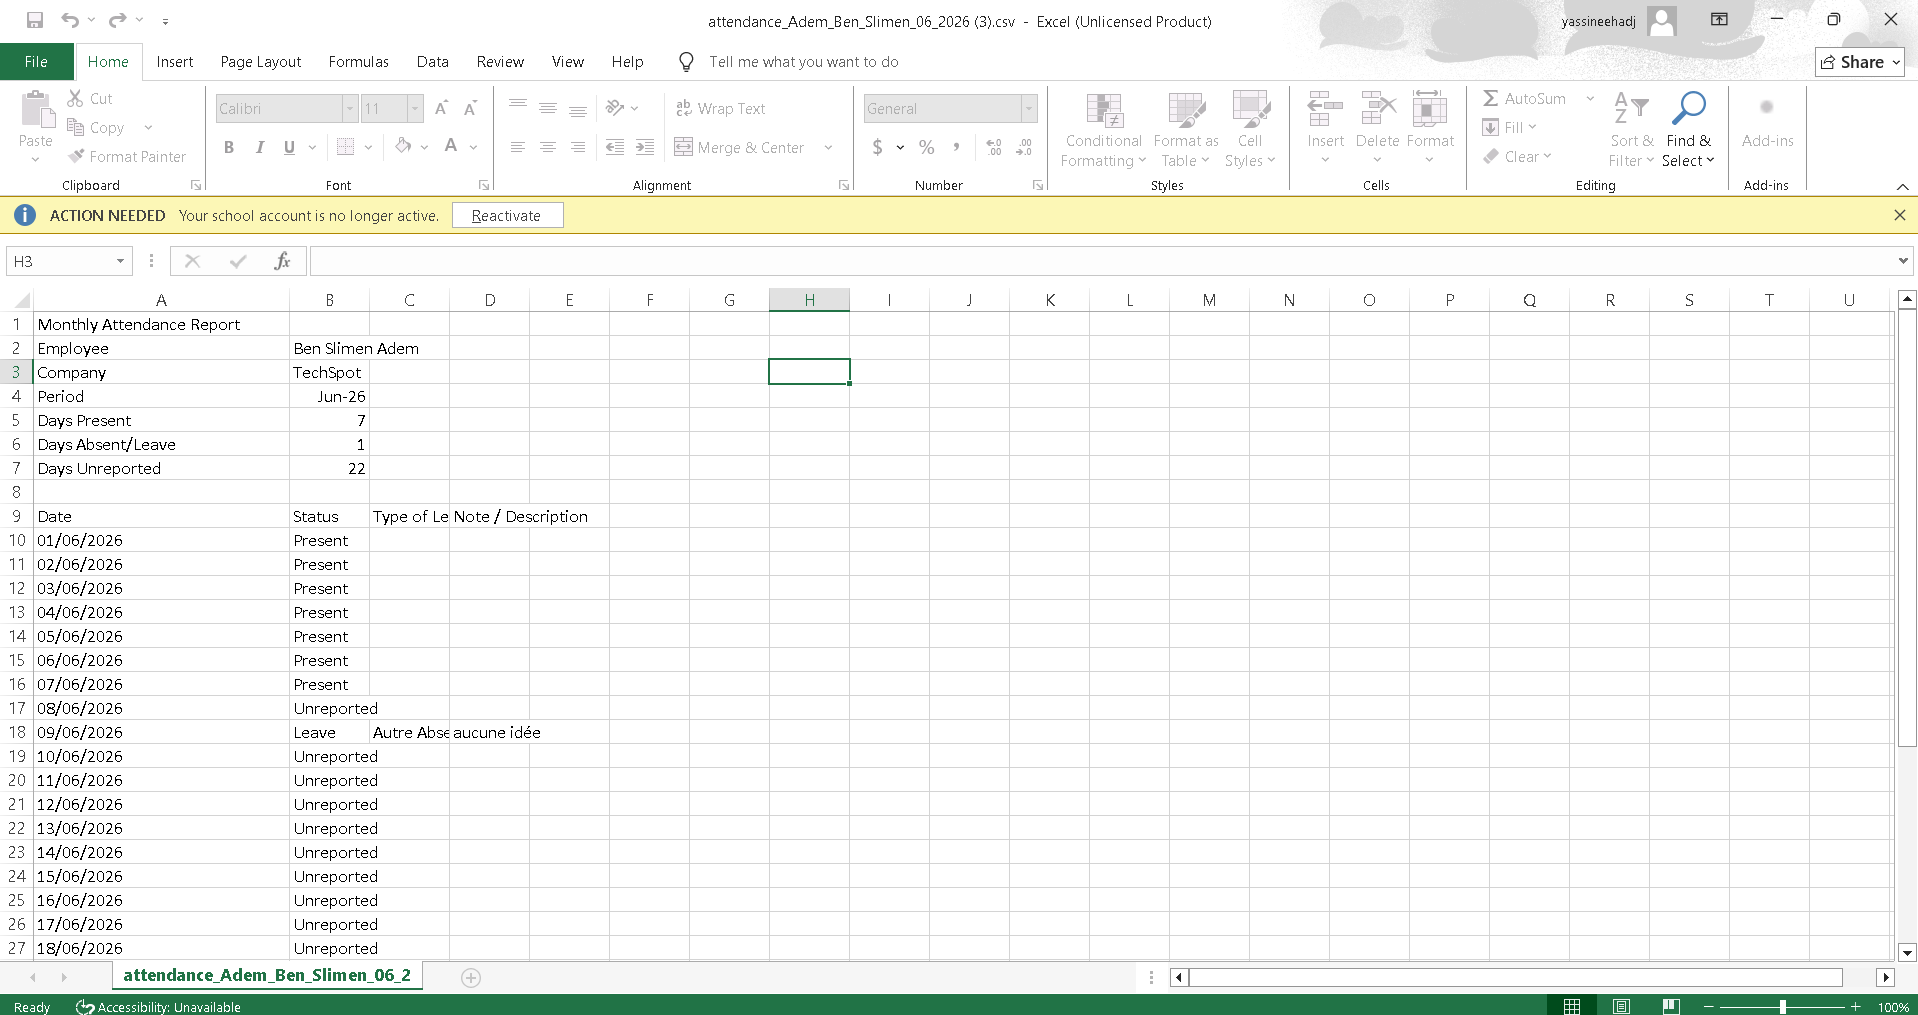
\includegraphics[width=0.85\textwidth]{project_images/eployee_attendance_file.png}
    \caption{Attendance Spreadsheet}
    \label{fig:out_excel}
\end{subfigure}
\caption{Application Output Files - PDF Export and Excel Attendance Spreadsheet}
\label{fig:output_demos}
\end{figure}


\subsection{Utility Evaluation}
The implemented features were thoroughly tested throughout the development process to ensure that they met the functional requirements of HMI Stars Consulting. Special attention was given to document management, employee tracking, attendance management, and communication features. The results confirmed that the system successfully supports the company's daily administrative operations in a centralized and efficient manner.

\subsection{Usability Evaluation}
Several tests were carried out to verify the usability and reliability of the application on both web and mobile platforms. The user interfaces were refined to provide a simple and intuitive experience, while real-time features such as messaging and notifications were validated to ensure smooth interactions. Authentication, navigation, and data synchronization processes were also tested to guarantee a stable and seamless user experience.

\section{Conclusion}
The testing and evaluation phases confirmed that the HMI Stars ecosystem is stable, secure, and fully meets all initial project requirements. The mobile application successfully delivers employee management, attendance tracking, leave requests, real-time messaging, document sharing with scanning capabilities, and disciplinary warning templates. The web platform provides a comprehensive administration workspace with company management, employee registries, document archives, warning systems, notes and reminders, and attendance export capabilities. Both components support bilingual interfaces (French and English) and adaptive themes (light and dark), ensuring accessibility and comfort for all users. The transition phase successfully configured and launched all components within their designated execution environments, confirming readiness for production deployment.
